% modificar la caratula

% falta analisis de resultados (que despues se replica en las conclusiones) ¿Que mas se puede poner?

% concluciones: presentamos una herramienta, analizamos los ejemplos para ver la ganacia obteniendo una mejora de 10 veces.
\documentclass[a4paper,	11pt]{report}
%-----------Paquetes-------------------------
\usepackage[utf8]{inputenc}
\usepackage{amsmath}
\usepackage{amssymb}
\usepackage[chapter]{minted}
\usepackage{todonotes}

\usepackage{xpatch,letltxmacro}
\LetLtxMacro{\cminted}{\minted}
\let\endcminted\endminted
\xpretocmd{\cminted}{\RecustomVerbatimEnvironment{Verbatim}{BVerbatim}{}}{}{}


\usemintedstyle{trac} 
\usepackage[hidelinks]{hyperref}
%\usepackage[lined,boxed,spanish,onelanguage]{algorithm2e} 
\usepackage{algorithm}
\usepackage{algpseudocode}
\usepackage{graphicx}
\usepackage[strict]{changepage}

\usepackage{booktabs}
\usepackage[outermargin=-4cm,]{fullwidth}
\usepackage{tikz}
\usepackage{smartdiagram}
\usetikzlibrary{trees}

\tikzstyle{every node}=[draw=black,thick,anchor=west]
\tikzstyle{selected}=[draw=red,fill=red!30]
\tikzstyle{optional}=[dashed,fill=gray!50]

\usepackage{mdframed}

\usepackage[spanish]{babel}
\renewcommand\listingscaption{Listado}

\newcommand\TBox[2][]{%
  \tikz\node[draw,ultra thick,align=left,#1] {#2};\hskip2pt}

\makeatletter
\newcommand*{\centerfloat}{%
  \parindent \z@
  \leftskip \z@ \@plus 1fil \@minus \textwidth
  \rightskip\leftskip
  \parfillskip \z@skip}
\makeatother

\begin{document}

\renewcommand\floatpagefraction{.9}
\renewcommand\topfraction{.9}
\renewcommand\bottomfraction{.9}
\renewcommand\textfraction{.1}
\setcounter{totalnumber}{50}
\setcounter{topnumber}{50}
\setcounter{bottomnumber}{50}
\newcommand{\quotes}[1]{``#1''}

\title{Conversión de modelos PowerDEVS al lenguaje Modelica}
\author{Tesinista: Luciano Andrade A-2121/1\\ Director: Federico Bergero, Co-Director: Ernesto Kofman} 


\begin{titlepage}
\begin{center}

\huge Conversión de modelos PowerDEVS al lenguaje Modelica

\vfill

Tesina de grado para la obtención del grado de Licenciado en Ciencias de la Computación

\begin{minipage}[t]{0.4\textwidth}
\begin{flushleft} \large
\emph{Tesinista :}\\
Luciano Andrade
\end{flushleft}
\end{minipage}\\ 
\vfill
\begin{minipage}[t]{0.4\textwidth}
\begin{flushleft} \large
\emph{Director :}\\
Federico Bergero
\end{flushleft}
\end{minipage}%
\begin{minipage}[t]{0.4\textwidth}
\begin{flushright} \large
\emph{Co-Director:} \\
Ernesto Kofman 
\end{flushright}
\end{minipage}

\vfill

\includegraphics[width=0.25\textwidth]{logo-unr}

\vfill

{\large \today}
\end{center}
\end{titlepage}


\tableofcontents

\begin{abstract}

El modelado y simulación se han convertido en una actividad centrales de todas las disciplina ingenieriles y científicas, son utilizados en el análisis de sistemas  ayudándonos a ganar un mejor entendimiento de su funcionamiento. 
Son importantes para el diseño de nuevos sistemas donde podemos predecir el comportamiento del sistema antes de que sea construido.
El modelado y simulación son las únicas técnicas disponibles que nos permiten analizar sistemas arbitrarios no lineales bajo una variedad de condiciones experimentales.

PowerDEVS es un entorno integrado para el modelado y simulación basada en el formalismo DEVS, permite definir modelos atómico en C++ que puede ser conectados gráficamente en bloques jerárquicos para crear sistemas más complejos. El entorno automáticamente transforma el modelo a código C++ que ejecuta la simulación.

QSS-Solver es una implementación independiente de los métodos de integración por cuantificación de estados (Quantized State System) para simulaciones de sistemas continuos e híbridos. Los métodos QSS remplazan la integración por discretización del tiempo por integración por cuantificación de estados del sistema (Quantized State System) y a diferencia de los sitemas DEVS no requiere los mecanismos de sincronización y transmición los eventos de los sistemas DEVS.

En este trabajo se presenta una aplicación capaz de convertir modelos, descriptos en PowerDEVS, en código Modelica, más específicamente código $\mu$-Modelica (un subconjunto de Modelica), permitiendo ejecutar este modelo (convertido) con alguno de los compiladores Modelica, OpenModelica o Dymola, o \quotes{QSS Solver}, este último nos permite ganar al menos un orden de magnitud en los tiempos incurridos en la simulación.

\end{abstract}


\chapter{Introducción}


While the scientist is happy to simply observe and understand the world, i.e., create a model of the world, the engineer wants to modify it to his or her advantage.

Let me state a number of good reasons for using simulation as a problem-solving tool.
(1) The physical system is not available. Often, simulations are used to determine whether a projected system should ever be built. So obviously, experimentation is out of the question. This is common practice for engineering systems (for example, an electrical circuit) with well-established and widely applicable meta-knowledge. It is very dangerous to rely on such a decision in the case of systems from soft sciences (the so-called ill-defined systems) since the meta-knowledge available for these types of systems is usually not validated for an extension into unknown territory.

(2) The experiment may be dangerous. Often, simulations are performed in order to find out whether the real experiment might "blow up," placing the experimenter and/or the equipment under danger of injury/ damage or death/ destruction (for example, an atomic reactor or an aircraft flown by an inexperienced person for training purposes).

(3) The cost of experimentation is too high. Often, simulations are used where real experiments are too expensive. The necessary measurement tools may not be available or are expensive to buy.
It is possible that the system is used all the time and taking it "off-line" would involve unacceptable cost (for example, a power plant or a commercial airliner).

( 4) The time constants (eigenvalues) of the system are not compatible with those of the experimenter. Often, simulations are performed because the real experiment executes so quickly that it can hardly be observed (for example, an explosion) or because the real experiment executes so slowly that the experimenter is long dead before the experiment is completed (for example, a transgression of two galaxies). Simulations allow us to speed up or slow down experiments at will.

(5) Control variables (disturbances), state variables, and/or system parameters may be inaccessible. Often, simulations are performed because they allow us to access all inputs and all state variables, whereas, in the real system, some inputs ( disturbances) may not be accessible to manipulation (for example, the time of sunrise) and some state variables may not be accessible to measurement. Simulation allows us to manipulate the model outside the feasible range of the physical system. For example, we can decide to change the mass of a body at will from 50  kg to 400 kg and repeat the simulation at the stroke of a key. In the physical system, such a modification is either not feasible at all or it involves a costly and lengthy alteration to the system.

(6) Suppression of disturbances. Often, simulations are performed because they allow us to suppress disturbances that are unavoidable in the real system. This allows us to isolate particular effects, and may lead to a better insight (intuition) into the generic system behavior than would be possible through obscured measurements taken from the real process.

(7) Suppression of second-order effects. Often, simulations are performed because they allow us to suppress second-order effects (such as nonlinearities of system components). Again, this can help with the understanding of the primary underlying functionality of the system.

% XXX explicar como se desarrolla un modelo en Modelica / µ-Modelica
% XXX explicar la como se desarrolla un modelo en PowerDEVS, 
% TODO explicar que el QSS Solver nos puede ahorrar un orden de magnitud en el tiempo de ejecución de la simulación

The Stand–Alone QSS solver presented here overcomes this problem, improving in more than one order of magnitude the computation times of the pre- vious discrete event implementations.
















En este trabajo se describe la implementación de una aplicación capaz de convertir modelos descriptos en la herramienta PowerDEVS\cite{BK11} a modelos en el lenguaje Modelica\cite{Fritzson02modelica--}, más específicamente en $\mu$Modelica\cite{Ber12}, en el primer capitulo presentamos las principales motivaciones y objetivos, así como trabajos relacionados y el alcance de este trabajo. En el capitulo dos se recorren conceptos previos, principalmente los formalismo DEVS implementados en PowerDEVS, es decir, DEVS parametrizado y DEVS Vectorial. En el capítulo tres se muestra en detalles el proceso de conversión de modelos, por ultimo, en el capitulo cuatro, vemos los resultados del trabajo comparando los tiempos de ejecución de los modelos originales y las versiones convertidas a $\mu$modelica.

\begin{figure}[H]
\centering
 \includegraphics[width=0.75\linewidth]{esquema}
 \caption{Esquema de conversiones}
 \label{fig:esquema}
\end{figure}

En la figura \ref{fig:esquema}, se muestran los dos principales estrategias (PowerDEVS y Modelica) para realizar una simulación. En el caso de PowerDEVS, el primer paso es convertir el sistema en diagramas de bloques, luego en DEVS, en PowerDEVSe el cual puede automáticamente convertirlo en C++ y luego obtener los resultados ejecutando este modelo. Desde la perspectiva de Modelica (o $\mu$modelica, debemos pasar el sistema a modelica (o $\mu$Modelica) y luego el compilador se encargara de generar código (usualmente C o C++) capaz de correr la simulación y obtener resultados.
El actual trabajo esta representado por la flecha que sale de PowerDEVS hacia $\mu$modelica, permitiendo especificar la simulación en diagramas de bloques y ejecutar la simulación en el solver QSS, en el lenguaje $\mu$modelica.

\section{Organización del presente trabajo}

\section{Motivación y Objetivos}
PowerDEVS\cite{BK11} es una herramienta de simulación de sistemas híbridos, basado en el formalismo DEVS\cite{Zeigler:2000:TMS:580780}, con una interfaz gráfica orientada a bloques, donde los bloques pueden ser conectados entre si, modificado sus parámetros, además permite conectarse con el entorno Scilab para poder utilizar expresiones y herramientas de cálculo provistas por este entorno.

La resolución de ecuaciones diferenciales ordinarias, requiere el uso de métodos de integración numérica. Todos los algoritmos tradicionales de integración se basan en la discretización de la variable independiente (que generalmente representa el tiempo).

Las rutinas que implementan estos algoritmos, se denominan solvers y existen gran variedad de implementaciones de los mismos en diferentes lenguajes de programación. Los Métodos de Integración Numérica QSS (Quantized State System), a diferencia de los métodos de integración tradicionales, realizan la discretización sobre las variables de estado. En consecuencia, convierten los sistemas continuos en sistemas de eventos discretos, y tienen grandes ventajas para simular sistemas con discontinuidades.

Si bien PowerDEVS, implementa la totalidad de los algoritmos de QSS, resultan ineficientes, dado que malgastan gran parte de la carga computacional en la transmisión de eventos entre submodelos.

Para solventar este hecho se desarrollo una familia de QSS stand-solver, el cual requiere un modelo descripto en lenguaje C el cual contiene las ecuaciones diferenciales, las funciones de cruce de cero así como la información estructural requerida por los algoritmos QSS. Estos solvers obtienen una mejora de rendimiento de hasta un orden de magnitud comparado con otras implementaciones DEVS.

Sobre este se desarrollo una herramienta la cual genera a partir de un modelo $\mu$-Modedelica \cite{Ber12} (un subconjunto del lenguaje Modelica) el modelo requerido para el QSS solver.

Con el objetivo de utilizar los mejoras de velocidad y mantener un entorno amigable con el usuario, se creo una herramienta capas de convertir un modelo PowerDEVS en un modelo $\mu$modelica.


\section{Trabajo relacionado}
En \cite{Ber12} se describe una extensión del Compilador OpenModelica el cual traslada modelos regulares Modelica a $\mu$modelica. 
ModelicaDEVS \cite{Beltrame06quantisedstate} es una librería Dymola que permite describir simulaciones DEVS en el Modelica, más específicamente en el entorno Dymola.
M/CD++ \cite{conf/mascots/DAbreuW05} es una herramienta para convertir simulaciones en un subconjunto de Modelica, a simulaciones DEVS.
DESlib \cite{Sanz09paralleldevs} es una librería para la descripción de modelos Parallel DEVS en Modelica.


\section{Alcance}
DEVS\cite{Zeigler:2000:TMS:580780}, Discrete Event System Specification (Especificación de Sistemas de Eventos Discretos), es un formalismo modular y jerárquico para modelar y analizar sistemas que pueden ser de eventos de tiempo discreto mediante tablas de transición, y con estados continuos que pueden ser descriptos por ecuaciones diferenciales.
En el formalismo clásico DEVS, los modelos atómicos capturan el comportamiento del sistema, mientras los modelos Acoplados describen la estructura del mismo.
En particular los modelos atómicos en PowerDEVS son descriptos en clases C++, mientras que la estructura se encuentra definida en archivos pds y pdm.
Modelica es un lenguaje de modelado, orientado a objetos, declarativo, para el modelado orientado a componentes de sistemas complejos.
Para poder realizar nuestro objetivo es necesario primero contar con un modelo en modelica\cite{Fritzson02modelica--} para cada atómico PowerDEVS\cite{BK11} que deseemos convertir. 

De esto se desprenden las siguientes limitaciones importantes:
\begin{itemize}
	\item La semántica de los modelos convertidos depende de los modelos equivalentes a los DEVS atómicos 
	\item Solamente podemos convertir modelos cuyos componentes atómicos hayan sido convertidos a $\mu$modelica.
\end{itemize}




\chapter{Conceptos Previos}
	En este capítulo, basado en \cite{Fer12}, \cite{Ber12Th}, \cite{BK11}, \cite{BK13}, introducimos algunos conceptos básicos de modelado y 
	simulación de sistemas, formalismos necesarios para poder comprender este trabajo. 

\section{Modelado y Simulación}
	El Modelado y Simulación\cite{Zeigler} de un sistema es el proceso por el cual se desarrolla un modelo, el cual es luego ejecutado, de forma de obtener datos 
	sobre el comportamiento del sistema.  El modelo debe conservar las principales características del sistema, pero al mismo tiempo ser significativamente 
	más simple, de forma que al momento de simularlo sea más eficaz utilizar la simulación que el sistema en sí.

	\subsection{Sistemas Continuos y Discretos}
	Se considera un sistema continuo si las variables de éste son conocidas en cada instante de tiempo, mientras que se considera discreto si las 
	variables son conocidas en instantes de tiempo determinados.

	En general, los sistemas en estudio serán continuos, pero deberemos utilizar sistemas discretos para simularlo, puésto que la simulación en 
	computadora así lo requiere, dado que la misma computadora es un sistema discreto.

	\subsection{Métodos de integración numérica} \label{sec:num_integ}
	Un sistema continuo puede ser descripto por una ecuación diferencial ordinaria de la forma:

	\begin{equation} \label{eq:eq1}
	\dot{x}(t) = f (x(t), u(t))
	\end{equation}
	donde $x \in \mathbb{R}^n$  es el vector de estados, $u \in \mathbb{R}^m$ es una función de entradas conocidas,
	$t$ representa el tiempo, y con sus condiciones iniciales:

	\begin{equation} \label{eq:eq2}
	x(t = t_0 ) = x_0
	\end{equation}

	Sea $x_i (t)$ la trayectoria del estado $i$-esimo expresada como función de tiempo simulado. 
	Mientras que la ecuación  \eqref{eq:eq1} no contenga discontinuidades $x_i (t)$ será una función continua con derivada continua. 
	Esta puede ser aproximada con la precisión deseada mediante series de Taylor en cualquier punto de su trayectoria.

	Denominando $t^{\ast}$ al instante de tiempo en torno al cual se aproxima la trayectoria mediante una serie de Taylor, y siendo $t^{\ast} + h$
	 el instante de tiempo en el cual se quiere evaluar la aproximación, entonces, la trayectoria en dicho punto puede expresarse como sigue:

	\begin{equation} \label{eq3}
		x_i(t^* + h) = x_i(t^*) + \frac{dx_i (t^*)}{dt} \cdot h + \frac{d^{2}x_i (t^*)}{dt^2} \cdot \frac{h^2}{2!} + \cdots
	\end{equation}

	Reemplazando con la ecuación de estado \ref{eq:eq1}, la serie \eqref{eq3} queda:

	\begin{equation} \label{eq4}
		x_i(t^* + h) = x_i(t^*) + f_i(t^*) \cdot h + \frac{d^{2}x_i (t^*)}{dt^2} \cdot \frac{h^2}{2!} + \cdots
	\end{equation}

	Los distintos algoritmos de integración difieren en la manera de aproximar las derivadas superiores de $f$ y en el número de
	 términos de la serie de Taylor que consideran para la aproximación, entre los principales métodos podemos mencionar Runge-Kutta\cite{Cel06}, DASSL\cite{DASSL}, DOPRI\cite{DP80}, etc.

\section{Un ejemplo}
	Introducimos un modelo de ejemplo, el cual mostraremos paso a paso, a lo largo de este trabajo, como se lleva adelante la transformación de modelos: 
	el sistema de ecuaciones de Lotka-Volterra, también conocidas como ecuaciones predador-presa o presa-predador,
	son un par de ecuaciones diferenciales de primer orden no lineales que se usan para describir la dinámicas de sistemas biológicos en el que dos 
	especies interactúan, una como presa y otra como depredador.
	\label{lotka_volterra_ref}

	\begin{align*}
		\frac{dx}{dt} &= x(\alpha - \beta y) \\
		\frac{dy}{dt} &= - y(\gamma - \delta  x)
	\end{align*}

	donde:
	\begin{itemize}
		\item $y$ es el número de algún predador (por ejemplo, un lobo)
		\item $x$ es el número de sus presas (por ejemplo, conejos)
		\item $\frac{dy}{dt}$ y $\frac{dx}{dt}$ representa el crecimiento de las dos poblaciones en el tiempo
		\item $t$ representa el tiempo
		\item $\alpha$, $\beta$, $\gamma$ y $\delta$ son parámetros que representan las interacciones de las dos especies.
	\end{itemize}

	

\section{Modelica}\label{sec:modelica}

	Modelica\cite{Fri98}\cite{Fritzson02modelica} es un lenguaje orientado a objetos desarrollado para describir de manera sencilla modelos de sistemas 
	dinámicos eventualmente muy complejos.
	Además de las características básicas de todo lenguaje orientado a objetos, contiene herramientas específicas que permiten describir las relaciones
	constitutivas de los distintos componentes de cada modelo y las relaciones estructurales que definen la interacción entre dichos componentes.
	De esta manera, el lenguaje permite asociar cada componente de un sistema a una instancia de una clase.
	Adicionalmente, los componentes típicos de los sistemas de distintos dominios de la física y de la técnica pueden agruparse en librerías de clases para ser
	reutilizados. De hecho, existe una librería estándar de clases de Modelica, que contiene los principales componentes básicos de sistemas eléctricos,
	mecánicos (traslacionales, rotacionales y multicuerpos), térmicos, state graph, y diagramas de bloques. 
	Otras librerías (disponibles en la web) contienen componentes de sistemas hidráulicos, bond graphs, redes de Petri, etc.
	Por otro lado, las herramientas que provee Modelica para expresar relaciones estructurales de un modelo permiten construir la estructura del mismo de una
	manera totalmente gráfica, lo que a su vez permite describir un sistema mediante un diagrama muy similar al del sistema físico idealizado.
	Como con todo lenguaje, para poder simular un modelo descripto en Modelica es necesario utilizar un compilador. Actualmente existen tres compiladores
	que implementan la mayoría del lenguaje Modelica: Dymola, MathModelica y OpenModelica. Los dos primeros son herramientas comerciales mientras que OpenModelica es de código
	abierto, todas cuentan con interfaces gráficas para construir los modelos, edición de código y compiladores para generar el código de las simulaciones.

\begin{listing}[H]    
	\inputminted[linenos]{modelica}{src/LotkaVolterra.mo}
	\caption{LotkaVolterra.mo}\label{lst:LotkaVolterra.mo}
\end{listing}
	
	Continuando con el ejemplo del sistema de ecuaciones de Lotka-Volterra, en el Listado \ref{lst:LotkaVolterra.mo} se muestra el modelo equivalente en Modelica, 
	en el se pueden observar algunas particularidades del lenguaje.
	
	En la línea 1 se puede ver el modelo, en este caso una \quotes{clase} y su nombre LotkaVolterra.
	Modelica, utiliza 7 clases restringidas:
	\textbf{block}, \textbf{connector}, \textbf{function}, \textbf{model}, \textbf{package}, \textbf{record} y \textbf{type}.
	Cada una de estas clases restringidas permite declarar clases más específicas y cualquiera de ellas puede reemplazarse
	por \textbf{class}, pero siempre es mejor especificar de que tipo de clase se trata para mejorar la legibilidad y facilitar la depuración de código.

	Las siguientes dos líneas declaran las variables \texttt{x} e \texttt{y} del tipo \texttt{Real}, ambas con valor de inicio \texttt{0.5}, las líneas 4 a 7, 
	declaran los parámetros \texttt{a}, \texttt{b}, \texttt{c} y \texttt{d} . A diferencia de \texttt{x} e \texttt{y}, estos parámetros no pueden cambiar durante la 
	simulación, pero pueden cambiar de simulación en simulación.

	Esta primera parte (líneas 2 a 7) del modelo constituye la sección de declaraciones a continuación, se encuentra la sección de ecuaciones 
	(luego de la palabra clave \texttt{equation}), esta sección describe el sistema de ecuaciones de nuestro modelo, donde la expresión \texttt{der(x)} 
	representa la derivada \texttt{x} respecto del tiempo y análogamente con \texttt{y}.
	
	Por supuesto Modelica es un lenguaje mucho más extenso de lo que hemos descripto, pero los conceptos que utilizamos a lo largo de este trabajo son los
	expresados en la presente sección.


\section{Métodos de integración QSS}
	Los métodos Quantized State System \cite{Fer12}\cite{Ber12}\cite{Beltrame06quantisedstate}\cite{Cel06}, pueden aproximar Ecuaciones 
	Diferenciales Ordinarias (ODE por sus siglas en inglés) mediante modelos de eventos discretos cuantificando los estados del sistema, 
	a diferencia de los métodos mencionados en la sección \ref{sec:num_integ}, los cuales realizan la integración sobre el tiempo. 

	Formalmente, el método QSS de primer orden (llamado QSS1) aproxima la ecuación \ref{eq:eq1} por:
	
	\begin{equation}
	\dot{x}(t) = f (q(t), v(t))
	\end{equation}
	donde $q$ es el vector de estados cuantificados y sus componentes están relacionadas una a una con las del vector de estados $x$ siguiendo una 
	función de cuantificación con histéresis:
	
	\begin{equation}
	q_j(t) = \left\{ 
	  \begin{array}{l l}
	    x_j(t)  \quad \text{si} \mid x_j (t ) - q_j (t^{-} ) \mid \geq \Delta Q_j \\
	    q_j (t^{-} ) \quad \text{en caso contrario}
	  \end{array} \right.
	\end{equation}
	
	donde $q_j (t^{-})$ es el límite por izquierda de $q_j$ en $t$.
	
	\begin{figure}[H]
	  \includegraphics[scale=0.5]{histeresis1}
	  \caption{Variables Relacionadas con una Función de Cuantificación con Histéresis de orden cero.}\label{fig:fig2-2}
	\end{figure}
	
	En la Figura \ref{fig:fig2-2} vemos la relación entrada-salida de una función de cuantificación de orden cero.
	
	Las variables $q_j$ son llamadas variables cuantificadas y pueden ser vistas como una aproximación constante por trozos de la variable de estado 
	correspondiente $x_j$. De la misma forma las componentes de $v(t)$ son aproximaciones constantes por trozos de las componentes correspondientes de $u(t)$. 
	Los pasos de integración en los métodos QSS sólo se producen cuando una variable cuantificada $q_j (t)$ cambia, esto es, cuando la variable de 
	estado correspondiente $x_j (t)$ difiere de $q_j(t^{-})$ en un quantum. Ese cambio implica también que algunas derivadas de estado (aquellas que 
	dependen de $x_j$ ) también son modificadas. 

	Luego, cada paso involucra un cambio en sólo una variable cuantificada y en algunas derivadas de estado. 
	Por lo tanto cuando un gran sistema sparse\footnote{Un sistema es sparse si posee sólo actividad en unos pocos estados mientras que el resto del sistema 
	se mantiene intacto}, los métodos QSS explotan intrínsecamente este hecho realizando cálculos sólo donde y cuando ocurren los cambios.
	Otra ventaja importante de los métodos QSS es que tratan las discontinuidades de una manera muy eficiente. Dependiendo del orden del método, 
	las variables de estado siguen trayectorias lineal por trozos, parabólica por trozos o constante por trozos, la ocurrencia de una discontinuidad implica 
	sólo algunos cálculos locales para re-computar las derivadas de estados que están directamente afectadas por ese evento.
	Estas ventajas resultan en una aceleración notable en el tiempo de simulación contra los algoritmos de integración numérica clásicos. 
	En modelos con discontinuidades frecuentes como sistemas de electrónica de potencia, los métodos de alto orden que veremos a continuación, 
	pueden simular hasta 20 veces más rápido que los métodos convencionales.


\section{$\mu$-Modelica}

	El lenguaje $\mu$-Modelica\cite{Ber12} se define como un subconjunto del lenguaje estandar Modelica, con las siguientes restricciones:

	\begin{itemize}
	 \item El modelo es plano, es decir no permite clases.
	 \item Todas las variables pertenecen al tipo predefinido Real y solo hay tres categorías de variables: estado continuo, estado discreto y variables 
	algebraicas.
	 \item Los parámetros también son de tipo Real. 
	 \item 
     
    Solo arreglos unidimensionales están permitidos, mientras que índices en los arreglos dentro de cláusulas \texttt{for} están restringidos a la forma $\alpha \cdot i + \beta$, 
	donde $\alpha$ y $\beta$ son expresiones enteras e \texttt{i} es el índice de la iteración.
	 \item La sección de ecuaciones está compuesta de:
	 \begin{itemize}
		\item Definición de variables de estados: $der(x) =  f (x(t), d, a(t), t);$ ODE en forma explícita
		\item Definición algebraica : $a_2  = g(a_1);$
	 \end{itemize}
	 con la restricción de que cada variable algebraica solo puede depender de variables estado y de variables algebraicas previamente definidas.
	 
	 \item Las discontinuidades son expresadas solo con las clausulas $when$ y $elsewhen$ dentro de la sección $algorithm$. Las condiciones dentro de las dos 
	clausulas solo pueden ser relaciones ($<$, $\leqslant$, $>$ $\geqslant$) y, dentro de la clausula, solo asignaciones de variables discretas y $reinit$ 
	de estados continuos son permitidos.
	\end{itemize}

	Estas restricciones son necesarias ya que el QSS-Solver necesita conocer la estructura del sistema para que luego de cada cambio de estado, solo deba evaluar
	las variables que explicitamente dependan de ella.

\section{Stand–Alone QSS solver}
	Como mencionamos antes los métodos QSS de integración reemplazan la discretización del tiempo de los métodos clásicos por una cuantificación de las 
	variables del sistema. De esta forma, estos métodos generan aproximaciones del sistema continuo y tienen algunas ventajas sobre sus contra partes clásicas.
	La forma más simple de implementar algoritmos QSS es mediante el uso de un simulador DEVS, de hecho PowerDEVS implementa la totalidad de la familia de 
	algoritmos QSS. Estas implementaciones aunque simples, son ineficientes, pues a diferencia de los sistemas DEVS no requieren de la sincronización y 
	transmisión de eventos, permitiendo liberar parte de la carga computacional.

	Estas desventajas motivaron el desarrollo del \emph{Stand–Alone QSS solver}\cite{Ber12}, implementado como un conjunto de módulos en lenguaje C. Este implementa 
	toda la familia de métodos QSS y permite que los modelos contengan discontinuidades de tiempo y estado.

	Un requerimiento impuesto por los métodos QSS es que hace uso de información estructural del modelo. Cada paso en un método QSS involucra un cambio 
	en una variable de estado y en la derivada del estado que depende de el. Debido a esto el modelo debe proveer no solo la expresión para calcular las 
	derivadas del estado (como en un clásico ODE solver) sino además una matriz de incidencias para informar al solver las que derivadas de estado han cambiado 
	luego de cada paso.

	Como sería muy incomodo para el usuario proveer esta información estructural, el solver tiene una interfaz que automáticamente obtiene la matriz de
	 incidencia desde una definición estándar de modelos.

	La interfaz permite al usuario describir el modelo utilizando ($\mu$-Modelica) y automáticamente genera el código C del modelo incluyendo la estructura.

	Continuando con nuestro ejemplo sobre el sistema Lotka Volterra, incluimos el modelo anterior, esta vez modificado para que sea $\mu$-Modelica valido.
	Se puede apreciar un bloque extra \texttt{initial algorithm} el cual inicializa las variables (en lugar de utilizar la inicialización estándar), además 
	fue necesario escribir las equaciones de la forma \texttt{var=f()} para que el modelo sean $\mu$-Modelica valido.

	\begin{listing}[H]    
		\inputminted[linenos]{modelica}{src/lotka_volterra_qss.mo}
		\caption{LotkaVolterra.mo}\label{lst:LotkaVolterra_qss.mo}
	\end{listing} 

\section{Formalismo DEVS}
	DEVS\cite{Zeigler} es un formalismo para modelar y analizar sistemas de eventos discretos (es decir, sistemas en los cuales en un lapso finito de tiempo, 
	ocurren una cantidad finita de eventos).
	Un modelo DEVS puede ser visto como un autómata que procesa una serie de eventos de entrada y genera una serie de eventos de salida. 
	Este procesamiento está regido por la estructura interna de cada una de las partes que componen el modelo general.
	Un modelo DEVS está descripto por dos clases de componentes, modelos atómicos y modelos acoplados.

	\subsection{Atómicos}
	Un modelo atómico representa la unidad \quotes{indivisible} de especificación, en el sentido que es la pieza fundamental y más básica de un modelo DEVS. 
	Formalmente un modelo atómico está conformado por la 7-upla:

	\begin{equation} 
	(X, Y, S, \delta_{int} , \delta_{ext}, \lambda, t_{a}) 
	\end{equation}
Donde:
	\begin{itemize}
	\item $X$ es el conjunto de valores de entrada que acepta el modelo atómico, es decir un evento de entrada tiene como valor un elemento del conjunto X.
	\item $Y$ es el conjunto de valores de los eventos de salida que puede emitir el modelo atómico.
	\item $S$ es el conjunto de estados internos del modelo, en todo momento el modelo atómico está en un estado dado, que es un elemento del conjunto S.
	\item $ta$ es una función $S \to \mathbb{R}^{+}_{0}$ , que indica cuánto tiempo el modelo atómico permanecerá en un estado dado, si es que no se recibe ningún 
	evento de entrada. Esta función se deonmina \emph{Función de Avance de Tiempo}.
	\item $\delta_{int}$ es una función $S \to S$, que indica la dinámica del sistema en el momento que el modelo atómico realiza una transición interna. 
	Sería el análogo a una tabla de transición en otros autómatas, es la \emph{Función de Transición Interna}.
	\item $\delta_{ext}$ es una función $(S \times \mathbb{R}^{+}_{0} \times X) \to S$, que indica el cambio de estado ante la presencia de un evento 
	externo, esta es la \emph{Función de Transición Externa}.
	\item $\lambda$ es una función $S \to Y$ llamada \emph{Función de Salida}, que indica qué evento se debe emitir al salir de un estado por una transición interna. 	\end{itemize}

	Los conjuntos $S$, $X$ e $Y$ son arbitrarios, y en general infinitos. Cada posible estado $s$ ($s \in S$) tiene asociado un Avance de Tiempo calculado 
	por la Función de Avance de Tiempo $ta(s)$.
	En la Figura \ref{fig:fig2-5} vemos la evolución de un modelo atómico. Si el estado cambia a $s_1$ en el tiempo $t_1$ , tras $ta(s_1)$ unidades de 
	tiempo (o sea, en tiempo $ta(s_1 ) + t_1 )$ el sistema realizará una transición interna cambiando a un nuevo estado $s_2$ dado por $s_2 = \delta_{int} (s_1 )$. 

	Cuando el estado va de $s1$ a $s2$ se produce un evento de salida con valor $y1 = \lambda(s1)$. La función $\lambda (\lambda : S \to Y )$.
	 Así, las funciones $ta$, $\delta_{int}$ y $\lambda$ definen el comportamiento autónomo de un modelo DEVS.

	Cuando llega un evento de entrada  el estado cambia instantáneamente. El nuevo valor del estado no sólo depende del valor del evento de entrada sino 
	también del valor anterior del estado y del tiempo transcurrido desde la última transición.

	Cuando llega el evento $x1$ en el instante $t3$ mientras se encuentra en el estado $s2$, despues de haber transcurrido el tiempo $e$ 
	(notar que $ta(s2 ) > e$) se transiciona al estado $s3 = \delta_{ext} (s2 , e, x1 )$ , luego de $ta(s_3)$ se transiciona a $s4$ y se emite el $y2$

	\begin{figure}[H]
	\centering
	  \includegraphics[scale=0.45]{devs-atomic}
	  \caption{Comportamiento de un modelo DEVS atómico}
	   \label{fig:fig2-5}
	\end{figure}


	\subsection{Acoplados}
	La descripción de un sistema puede ser completamente realizada utilizando un modelos atómico, aunque esto resulta un poco incómodo y confuso. 
	Los conjuntos de estados y las funciones de transición se vuelven inmanejables en sistemas complejos, y nunca podemos asegurar haber cubierto todos 
	los posibles estados.

	\begin{figure}[H]
	\begin{minipage}{0.5\textwidth}
	\centering
	\TBox{%
	  \TBox[]{Acoplado2 \\ \TBox{Acoplado1 \\ \TBox[]{Atómico1}\TBox{Atómico2} } \TBox{Atómico3} }}
	\end{minipage}\hfill
	\begin{minipage}{0.5\textwidth}
	\centering

	\begin{tikzpicture}[%
	  grow via three points={one child at (0.5,-0.7) and
	  two children at (0.5,-0.7) and (0.5,-1.4)},
	  edge from parent path={(\tikzparentnode.south) |- (\tikzchildnode.west)}]
	  \node {Root-Coordinator}
	    child { node {Acoplado2}		
	    child { node {Acoplado1}
	      child { node {Atómico1}}
	      child { node {Atómico2}}
	    }
	    child [missing] {}				
	    child [missing] {}				
	    child [missing] {}				
	    child { node {Atómico3}}};
	\end{tikzpicture}
	\end{minipage}

	\caption{Ejemplo de un modelo jerárquico.}\label{jerarquia}

	\end{figure}

	A modo de ejemplo, se puede ver en la Figura \ref{jerarquia} una jerarquía mostrando las relaciones entre los modelos acoplados y atómicos.

	Para abordar este problema, el formalismo DEVS introduce lo que se llaman modelos acoplados, que es una forma de agrupar modelos DEVS y generar 
	nuevos modelos a partir de este agrupamiento.
	Hay dos formas de acoplamiento, la más general, en la cual se utilizan funciones de traducción entre los sub–sistemas y otra clase que adopta el 
	uso de puertos para la comunicación entre sub–sistemas. Aunque estas dos formas son equivalentes entre sí, describiremos la segunda clase, ya que 
	es la más simple y es la utilizada en el presente trabajo.
	Formalmente un modelo acoplado está representado por la octo-upla:

	\begin{equation}
	N = (X_N , Y_N , D, {M_d }, EIC, EOC, IC, Select)
	\end{equation}

	donde cada componente es:
	\begin{itemize}
	\item $X_N$ es el conjunto de eventos de entrada al modelo acoplado, representado por el producto cartesiano del conjunto de puertos de entrada $InPorts$ y
	 el conjunto de posibles valores para cada puerto. O sea un evento de entrada al modelo acoplado está representado por un par $(p, v)$ donde 
	$p \in InPorts$ y $v \in X_p$ .

	\item $Y_N$ es el conjunto de eventos que el modelo acoplado puede emitir, representado por el producto cartesiano del conjunto de puertos de salida 
	$OutPorts$ y el conjunto de posibles valores para este puerto, o sea un evento de salida del modelo acoplado está representado por un par $(p, v)$ donde 
	$p \in OutPorts$ y $v \in Y_p$.

	\item $D$ es el conjunto de los índices a los modelos DEVS (atómicos y acoplados) que conforman este modelo. 

	\item ${M_d}$ con $d \in D$, es el conjunto de los modelos atómicos y/o acoplados (son justamente los modelos que \quotes{acopla} o \quotes{agrupa} 
	este modelo acoplado).

	\item EIC y EOC son los conjuntos de conexiones entre los modelos internos y los puertos del modelo acoplado:
	      \begin {itemize}
		  \item EIC (o External Input Coupling) son las conexiones de entrada al acoplado, es decir, conecta un puerto de entrada del acoplado con un 
			puerto de entrada de un modelo perteneciente al acoplado.
		  \item EOC (o External Output Coupling) son las conexiones de salida del acoplado. Conecta un puerto de salida de un modelo interno del
			 acoplado con un puerto de salida del acoplado.  
	     \end{itemize}

	\item $IC$ representa las conexiones internas del modelo acoplado.

	\item Select es una función $(\mathcal{P}((D)) \to D)$ que decide qué modelo realizará primero su transición interna, si se da el caso de 
		eventos simultáneos. Es una función de \quotes{desempate} que en ciertos modelos es necesaria.
	\end{itemize}

	Formalmente:
	\begin{align*}
	EIC \in& \{((N, ip_N ), (d, ip_d )) | ip_N \in InPorts, d \in D, ip_d \in InPorts_d \} \\
	EOC \in& \{((d, op_d ), (N, op_N ))  | op_N \in OutPorts, d \in D, op_d \in OutPorts_d \}
	\end{align*}
	donde N es el modelo acoplado.
	\begin{equation*}
	IC \in \{((a, ip_a ), (b, ip_b )) | a, b \in D, ip_a \in OutPorts_a , ip_b \in InPorts_b \}
	\end{equation*}
	donde no se permite que $a = b$.

	$InPorts$ y $Outports$ son conjuntos que describen los posibles puertos de entrada y salida respectivamente. En general se utilizan números enteros 
	para representar los puertos posibles por lo cual $InPorts = \mathbb{N}$ y $Outports = \mathbb{N}$. Los modelos acoplados son en sí mismos modelos 
	DEVS válidos; formalmente el acoplamiento (como lo definimos antes) es una operación cerrada sobre el conjunto de modelos DEVS. Acoplar modelos DEVS 
	forma nuevos modelos DEVS. Sin esta cualidad el acoplamiento resultaría inútil desde del punto de vista del formalismo. También trae muchas ventajas 
	a la hora de describir modelos DEVS y a la hora de simularlos. El acoplamiento da lugar a una estructura jerárquica de desarrollo.

	$EIC$, $EOC$ y $IC$ son conjunto de pares, de pares, como se encuentran conectados los modelos (atómicos o acoplados) a través de sus puertos con los 
	puertos de entrada, salida y con otros modelos (atómicos o acoplados) respectivamente. Tanto los puertos como los modelos son señalados por números 
	dentro de PowerDEVS, por lo que estos conjuntos estan comprendidos por elementos de la forma $(m_a, p_a), (m_b, p_b)$, donde $m_a$ y $m_b$ 
	son modelos (atómicos o no) en el actual modelo y $p_a$ y $p_b$ son sus correspondientes puertos.


	\subsection{Modelos DEVS parametrizados}
	Definiremos primero los modelos DEVS parametrizados\cite{BKC12} como un paso previo hacia el formalismo DEVS vectorial (Vectorial DEVS o VECDEVS), 
	el cual es una herramienta que nos facilitará representar modelos de gran escala en forma gráfica, en particular este formalismo se encuentra implementado 
	en la herramienta PowerDEVS.

	Formalmente : dado un modelo DEVS atómico $M$ obtenemos un Modelo DEVS Parametrizado:
	\begin{equation}
	M (p) = \{X, Y, S, \delta_{int}, \delta_{ext} ,\lambda , ta, p\}
	\end{equation}

	donde $p \in P$ es un parámetro que pertenece a un conjunto de parámetros arbitrario tal que $\delta_{int}$ , $\delta_{ext}$ , $\lambda$ y $ta$ 
	dependen también de $p$.
	Notar que dos modelos DEVS $M (p_1 )$, $M (p_2 )$ con $p_1 \neq p_2$ pueden exhibir distintos comportamientos aunque compartan los mismos conjuntos 
	de entrada, salida y de estados ($X$, $Y$ , y $S$, respectivamente).

	\subsection{Modelos Vectoriales}
	Dado el modelo escalar DEVS Parametrizado:
	\begin{equation}
		M (p) = \{X, Y, S, \lambda_{int} , \lambda_{ext} , \lambda, ta, p\}
		\end{equation}

		definimos un modelo Vectorial DEVS\cite{BKC12} como la estructura:
		\begin{equation}
		V_D = \{N, X_V, Y_V, P, \{M_i\}\},
		\end{equation}
		donde:
		\begin{itemize}
		\item $N \in \mathbb{N}$ es la dimensión del modelo vectorial.

		\item $X_V = X \times Index \bigcup \{-1\}$ es el conjunto de eventos de entradas vectorial donde $X$ es el conjunto de eventos de entrada del modelo 
		escalar e $Index = {1, \ldots , N }$ es el conjunto de índices que indican cuál de los modelos DEVS atómicos recibirá el evento.

		\item $Y_V = Y \times Index$ es el conjunto de eventos de salida vectorial donde $Y$ es el conjunto de eventos de salida del modelo escalar e 
		$Index = {1, \ldots , N }$ es el conjunto de índices que indica que modelo escalar de los $N$ , emitió el evento. 

		\item $P$ es un conjunto de parámetros arbitrario.

		\item Para cada índice $i \in Index$, $p(i) \in P$ es un parámetro y $M_i = M (p(i))$ es el modelo DEVS Parametrizado escalar.
	\end{itemize}

	\subsubsection{Interfaz entre DEVS Vectorial y DEVS}
	Para conectar bloques vectoriales y bloques escalares es necesarios bloques que hagan de interfaz entre los dos formalismo, además, introducimos 
	un bloque necesario para realizar modelos más complejos y conectar los diferentes componentes de un modelo vectorial entre sí.

	\begin{itemize}
		\item Escalar a Vector (Scalar to Vector): Este bloque simplemente agrega al índice $i$ al evento escalar que recibe, transformándolo en un 
			evento vectorial. Este modelo también posee un comportamiento especial para enviar el mismo evento en todas las componentes vectorial 
			al mismo tiempo, cuando $i = -1$, cada evento de entrada es trasmitido para todas las componentes del vector salida.
		\item Vector a escalar (Vector to Scalar): Este bloque tiene un parámetro $i$ que contiene el índice del vector de eventos a retransmitir, 
			cuando recibe un evento con indice $j=i$, remueve el indice y retransmite el evento escalar.
		\item Index Shift: El modelo más simple es el Index Shift. Cuando se recibe un evento con el valor $(x,i)$, emite un evento de salida $(x, i+sh)$, 
			donde $sh$ es un parámetro entero.
	\end{itemize}

	Es importante ver que los mensajes entre bloques vectoriales es un par donde uno de sus componentes es un número natural, que funciona como índice,
	el cual nos permite determinar en que posición del vector se encuentra la otra componente.

	En este trabajo todos estos bloques se la ha agregado la dimensión $N$ como parámetro, esto es necesario para realizar la conversión de los modelos,
	 de forma que no existan desconexiones a nivel Modelica, lo cual se reflejaría en un modelo con menos ecuaciones que variables, es decir un modelo 
	no balanceado.
	 
\section{PowerDEVS}
	PowerDEVS\cite{BK11}  es un programa, concebido para ser utilizado por expertos programadores DEVS, así como usuarios finales que solo quieren 
	conectar bloques y simular.

	\begin{figure}[!htbp]
	  \includegraphics[width=\textwidth]{powerdevs}
	  \caption{Interfaz gráfica de PowerDEVS}
	   \label{fig:powerdevsgui}
	\end{figure}

	PowerDEVS esta compuesto por varios programas independientes:
	\begin{itemize}
		\item El \emph{editor de modelos}, es desde el punto de vista del usuario, el principal programa de PowerDEVS, pues provee la interfaz gráfica 
			y enlaces para las demás aplicaciones. 
		Además de construir, manejar modelos y librerías, permite lanzar las simulaciones (lanzando el \emph{Pre procesador}) y editar los bloques 
		elementales hasta su definición atómica de modelo (invocando el \emph{Editor Atómico}).
		La ventana principal de \emph{Editor de Modelo} permite al usuario crear y abrir modelos y librerías. También permite a las librerías ser 
		exploradas y los bloques arrastrados de las librerías a los modelos.
		La ventana del Modelo provee todas las funcionalidades típicas para la edición gráfica para poder copiar, cambiar el tamaño, rotar, etc. mientras 
		que las conexiones pueden ser dibujadas entre los diferentes puertos.
		La ventana de Edición de Bloques, nos permite configurar la apariencia gráfica y elegir los parámetros del bloque y, en el caso de los modelos 
		atómicos, seleccionar el archivo que contiene el código asociado con la definición DEVS.

		\item El \emph{Editor de Modelos Atómicos} facilita la edición del código C++ correspondiente a cada modelo atómico DEVS, el usuario debe 
		definir las variables que forman el estado y parámetros y 6 funciones en sus correspondientes solapas, Init, Time Advance, Internal transition, 
		External transition, Output y Exit  
		Cuando el modelo se guarda, el código es guardado en los archivos .cpp y .h. 

		\item El \emph{Pre procesador}, toma un archivo .pdm (o .pds) producido por el \emph{Editor de Modelos} y produce el programa que corre 
		la simulación. Básicamente traduce el archivo .pdm a un archivo de cabecera .h que enlaza el simulador y el coordinador de acuerdo a la 
		estructura del modelo pasando además los parámetros definidos para el modelo.
		El \emph{Pre procesador}, además produce un Makefile (Makefile.include) el cual invoca el compilador para generar el programa que implementa 
		la simulación.

		\item La \emph{interfaz de simulación}, que corre el programa que implementa la simulación y permite variar parámetros de la simulación 
		como tiempo final, números de simulación a ejecutar, y el modo de simulación (normal, cronometrada, pasa o paso, etc.).

		\item Una instancia de Scilab, que actúa como un espacio de trabajo, donde los parámetros pueden ser leídos, y los resultados pueden ser exportados.
	\end{itemize}


	En la Figura \ref{fig:lk-powerdevs} se puede ver el modelo Lotka Volterra que acompaña la instalación de PowerDEVS, este modelo (aunque no visible en la Figura)
	tiene valores iguales a los expresados en el modelo equivalente anteriormente presentado en el Listado \ref{lst:LotkaVolterra.mo}. 
	Las dos conexiones contra el bloque \texttt{GnuPlot 0} representando las variables \texttt{x} e \texttt{y} es decir presa y depredadores, ambas variables 
	son el resultado de la integración por lo que los integradores \texttt{QSS Integrato 0} y \texttt{QSS Integrato 1} contienen en sus puerto de entrada los 
	valores \texttt{dx/dt} y \texttt{dy/dt}. 
	Los bloques \texttt{WSum 0} y \texttt{WSum 1}, tiene constante de forma que el valor de salida (\texttt{y}) queda definido como
	$y = K[0] * u0 + K[1] * u1 + \dots + K[7] * u7$ y en nuestro modelo son $K[0] = 0.1$ y $K[1] = -0.1$ en ambos bloques \texttt{WSum 0} y \texttt{WSum 1}.
	Replicando nuestra la ecuación de nuestro modelo.
	

	\begin{figure}[!htbp]
	  \includegraphics[width=\textwidth]{lk-powerdevs}
	  \caption{Modelo Lotka Volterra descripto en PowerDEVS}
	   \label{fig:lk-powerdevs}
	\end{figure}



\chapter{Conversión de modelos DEVS}
	En este capitulo describimos en detalles los pasos para realizar la transformación, utilizaremos el modelo ya presentado e introduciremos un modelo PowerDEVS con componentes
	vectoriales con el fin de ilustrar la transformación de estos componentes.

\section{Modelos DEVS}

        \subsection{Archivos PDS}
        PowerDEVS trabaja principalmente con dos archivos, .PDM y .PDS.
        Los archivos PDM es utilizado por el editor de modelos, pues contiene información estructural, así como información de posición de los modelos dentro del 
        editor, sus parámetros, lo cual indica nombre, tipo y valor, descripción de los modelos, la cantidad de puertos de cada modelo y las conexiones
        entre los modelos, los detalles de como esas conexiones son visualizadas por lineas y los detalles del recorrido de esas lineas. 
        Todos estos elementos son utilizados en primera medida con el editor de modelos, pero tambien son utilizados para generar el archivo PDS el cual es el 
        genera el código de la simulación.
        El archivo PDS contiene información estructural del modelo necesaria para realizar la simulación, en el listado \ref{lst:pdsstruc} se pueden ver un 
        esbozo de su estructura.
        
\begin{listing}[H]
\begin{minted}{text}
Root-Coordinator
 {
  Simulator
   {
    Path = vector\qss_sum_vec.h
    Parameters = "1","-1","1","0","0","0","0","0",3.000000e+00,"N"
   }
   ...
    Coordinator
     {
      ...
     }
   ...     
  Simulator
   {
        ...
   }
  EIC
   {
   }
  EOC
   {
   }
  IC
   {
        ...
   }
 }
\end{minted}
\caption{Estructura de un archivo PDS.}
\label{lst:pdsstruc}
\end{listing}

        Se puede observar un elemento \texttt{Root-Coordinator} el cual contiene (marcado entre llaves) una lista de \texttt{Simulator} que representan 
        los modelos atómicos y/o \texttt{Coordinator} que representan los modelos acoplados y tres listas de 
        conexiones \texttt{EIC}, \texttt{EOC} y \texttt{IC}, conexiones de entrada externa (External Input Connections), 
        conexiones de salida externa (external output connections) y conexiones internas (Internal Connections).

        Las lista de conexiones internas (IC) es una lista de par de pares de números naturales, de la forma $(a,b);(c,d)$.
        Donde el primer par se refiere al origen de la conexión (puerto $b$ de salida) del modelo $a$ y el segundo al fin de la conexión (puerto $d$ de entrada) 
        del modelo $c$, ambos modelos se refiere a la lista de modelos (atómicos o acoplados) del actual modelo.
        Es decir el par $(0,0);(1,0)$ indica que el puerto $0$ del segundo modelo (posición 1) es de entrada  y esta conectado al puerto $0$ del primer modelo.

        Tanto EIC y EOC siguen el mismo patron excepto que replazan el modelo de los puertos de salida y extrada respectivamente por $0$. Es decir el elemento 
        $(6,0);(0,1)$ en EOC indica que el puerto $0$ del modelo $6$ (septima posición)  se encuentra conectado con el puerto $1$ de salida del modelo 
        acoplado, y un par $(0,0);(2,1)$ en EIC indica que el primer puerto (puerto $0$) se encuentra conectado con el modelo 2 (tercera posición) en su puerto $1$.

        Los modelos acoplados dado que también son modelos DEVS, replican la estructura listado \ref{lst:pdsstruc}.

        Para poder leer esta estructura se cuenta con la librería de PowerDEVS\footnote{http://sourceforge.net/p/powerdevs/code/HEAD/tree/} la cual nos permite acceder
        a la estructura desde C++. 

\section{Modelos Atómicos}
        
        Internamente los modelos atómicos son identificados por el parámetro \texttt{Path} en el archivo PDS, para realizar la tradución de este modelo se utiliza 
        un modelo Modelica el cual debe seguir la siguiente especificación:

\begin{itemize}
        \item El código debe ser Modelica ($\mu$-modelica) valido y estar ubicado en el mismo directorio (y nombre del archivo) del código C que el modelo atómico 
        PowerDEVS, con el mismo nombre que el archivo .h, pero con extensión .mo, es decir un modelo con \texttt{vector\textbackslash qss\_sum\_vec.h} utilizara un modelo 
        \texttt{vector/qss\_sum\_vec.h} \footnote{El nombre de los archivos se replaza \quotes{\textbackslash} por \quotes{/} para permitir algunos modelos 
        cuyos \texttt{Path} contiene ese separadores de directorios}
        \item Los parámetros del modelo DEVS deben ser pasado en el parámetro $p$
        \item Los valores de entrada del modelo son asociados a la variable $u$
        \item Los valores de salida del modelos son asociados a la variable $y$
\end{itemize}

        Por ejemplo el código del integrador, originalmente ubicado en el archivo qss\_integrator.h de PowerDEVS, se ubica en el archivo qss\_integrator.mo mostrado en el listado 
        \ref{lst:qssintegrator.mo} ambos dentro del directorio qss.

\begin{listing}[H]
\begin{minted}{modelica}
class QSSIntegrator
  parameter Real p[4]={0,0,0,0,0,0,0,0};
  parameter Real x0 = p[4];
  Real u[1];
  Real y[1](start = {x0});
equation
  der(y[1]) = u[1];
end QSSIntegrator;
\end{minted}
\caption{Modelo qss\_integrator.mo}
\label{lst:qssintegrator.mo}
\end{listing}

        El modelo Lotka Volterra cuenta con dos integradores (con los mismo parámetros) representados en el listado \ref{lst:qssint.pds}, en este se puede ver 
        el valores de \texttt{Path} y \texttt{Parameters} que componen todos los modelos atómicos (por supuesto con los valores diferentes).

\begin{listing}[H]
\begin{minted}{text}
  ...
  Simulator
   {
    Path = qss/qss_integrator.h
    Parameters = "QSS3","1e-6","1e-3","0.5"
   }
   ...
\end{minted}
\label{lst:qssint.pds}
\caption{Extracto del modelo Lotka Volterra, modelo atómico de un integrator.}
\end{listing}

        Luego de remplazar los parámetros en la variable \texttt{p}, se prefijan todas las variables del modelo\footnote{La única variable que no se prefijada 
        es \texttt{time}} por el nombre del modelo y su posición en este caso con el prefijo 
        \quotes{\texttt{QSSIntegrator\_1\_}}, de esta forma podremos combinar varios modelos atómicos de forma que no existan \quotes{colisión} de nombres de variables,
        es decir dos variables de distintos modelos atómicos con el mismo nombre en Modelica. 

\begin{listing}[H]
\begin{minted}{modelica}
class QSSIntegrator
  parameter Real QSSIntegrator_1_p[4]={0,1e-6, 1e-3, 0.5};
  parameter Real QSSIntegrator_1_x0 = p[4];
  Real QSSIntegrator_1_u[1];
  Real QSSIntegrator_1_y[1](start = {QSSIntegrator_1_x0});
equation
  der(QSSIntegrator_1_y[1]) = QSSIntegrator_1_u[1];
end QSSIntegrator;
\end{minted}
\caption{Transformación parcial de un modelo atómico de un integrator en el modelo de ejemplo Lotka Volterra.}
\end{listing}

        Los parámetros son remplazados en el modelo, evaluándolos en Scilab\footnote{Para realizar la evaluación en Scilab se utiliza el mismo mecanismo que 
        provee (y utiliza) PowerDEVS.}, lo que los transforma en float, los cuales son presentados como reales (Real) en el código.

        Los modelos (atómicos) no encontrados son ignorados en la traducción y se reportan en el registro (archivo .log) de la conversión.

        Esta transformación se repite para todos los modelos atómicos del archivo .PDS dentro del \texttt{Root-Coordinator}, los modelos acoplados 
        (dentro de un \texttt{Coordinator}) deben ser transformados a un conjunto de atómicos equivalentes.
        \quotes{Plano}

\section{Modelos Acoplados Planos}

        Llamamos \emph{Modelos Acoplados Planos} a los Modelos que solo contienen \emph{Modelos Atómicos}. Es decir que no contienen Modelos acoplados.

        Cada uno de los modelos atómicos que incluye se transforma de la misma forma que describimos en la sección anterior y dado que no existen \quotes{colisiones} 
        de nombres variables, podes combinar las diferentes secciones en un modelo compuesto el cual tendra todas las secciones \texttt{equation}, \texttt{initial equation} y declaraciones.
        Luego cada conexión entre Modelos Atómicos es replicada en el código de Modelica resultante. Los modelos Atómicos cuyo entrada (o salida) son escalares son conectados con un ecuación 
        del tipo $u = y$ mientras que los modelos vectoriales son conectados con la misma ecuación, solo que dentro de un \texttt{for}.

\begin{listing}[H]
        \inputminted[linenos]{modelica}{src/lotka_volterra-orig.mo}
        \caption{Modelo Lotka Volterra convertido de PowerDEVS a $\mu$-Modelica}
        \label{lst:lotka_volterra-orig.mo}
\end{listing}

        En el listado \ref{lst:lotka_volterra-orig.mo} se puede ver el resultado de la conversión del modelo Lotka Volterra, en el se puede apreciar en las líneas 
        2 a 21 correspondientes a las declaraciones de las variables de los modelos atómicos y de las líneas 22 a 27 correspondientes a las ecuaciones de estos 
        modelos y de la línea 28 a 35 son las ecuaciones correspondientes a las conexiones entre modelos atómicos.

        En las lineas de conexiones (28 a 35) se puede ver como se utilizan las variables \texttt{u} e \texttt{y} (prefijadas con sus correspondientes modelos
        atómicos y posición). Tanto los puertos de entrada, \texttt{u}, como los puertos de salida, \texttt{y}, son representados en Modelica como arreglos,
        permitiendo a modelos que cuentan con más de un puerto reflejar este hecho, asociando cada puerto con la posición correspondiente del arreglo. 
        cabe mencionar que existe un desfase, ya que los puerto en PowerDEVS son enumerados desde el cero, mientras que Modelica inician los arreglos de uno, por lo
        que el puerto $n$ corresponde a la variable $u[n+1]$ si es un puerto de entrada y $y[n+1]$ si es un puerto de salida.

        En el ejemplo Lotka Volterra no hay modelos atómicos vectoriales, veremos más adelante un ejemplo, pero es oportuno mencionar que los modelos
        vectoriales difieren en la forma en que se conectan, dado que la conexión debe realizarse iterando, con un \texttt{for}, sobre la primera dimensión del 
        arreglo que representa el puerto, en el caso escalar, que es el caso por omisión, solo alcanza con igualar las variables mencionadas.


\section{Modelos Acoplados Jerárquicos}
        En la sección anterior mostramos como son convertidos modelos acoplados planos, para convertir un modelo acoplado jerárquico, es decir un modelos con más 
        modelos acoplados internos, vamos a generar un modelo acoplado plano, equivalente al modelo jerárquico inicial.

        Para realizar el aplanado, se recorre recursivamente los modelos acoplados:

        \begin{itemize}
                \item por cada modelo acoplado si solo tiene modelos atómicos, es remplazado por los modelos atómicos internos, los cuales se encuentran conectados 
                        sin modificaciones excepto por las conexiones externas, las cuales son reasignadas de forma de mantener las conexiones.
                \item si el modelo acoplado contiene otros modelos acoplados entonces aplanamos ese modelo recursivamente.
        \end{itemize} 

        De esta forma obtenemos un modelo con solo modelos atómicos el cual podemos convertir con el procedimiento anteriormente descripto.

\begin{figure}[H]
        \begin{minipage}{0.5\textwidth}
        \includegraphics[width=\linewidth]{buck_disk}
        \end{minipage}
        \begin{minipage}{0.5\textwidth}
        \includegraphics[width=\linewidth]{buck_disk_coupled0}
        \end{minipage}
 \label{fig:coupledsample}
 \caption{Ejemplo de Modelo acoplado(derecha), junto a una detalle del modelo \texttt{Coupled0}}
\end{figure}

        En la figura \ref{fig:coupledsample}  se observa a la derecha el modelo de un convertidor Buck (o reductor) es un convertidor de potencia, 
        el cual introduciremos con mayores detalles en una sección posterios, y a la izquierda el modelo acoplado \texttt{Coupled0}.

\begin{figure}[H]

  %\setcapwidth{0.6\textwidth}
  \makebox[\textwidth][c]{%
        \begin{minipage}[t][][b]{.59\textwidth}
        \begin{tikzpicture}[%
          grow via three points={one child at (0.5,-0.7) and
          two children at (0.5,-0.7) and (0.5,-1.4)},
          edge from parent path={(\tikzparentnode.south) |- (\tikzchildnode.west)}]
          \node {Root-Coordinator}
            child { node {Scilab Command0}}             
            child { node {QSS Integartor0}}
            child { node {QSS Integartor1}}             
            child { node {Coupled0}
              child { node {WSum0}}
              child { node {Inseverse0}}
              child { node {Multiplier0}}
              child { node {Multiplier1}}
              child { node {Multiplier2}}
              child { node {Inseverse1}}
              child { node {Multiplier3}}
              child { node {Multiplier4}}
              child { node {WSum1}}
            }
            child [missing] {}                          
            child [missing] {}                          
            child [missing] {}                          
            child [missing] {}                          
            child [missing] {}                          
            child [missing] {}                          
            child [missing] {}                          
            child [missing] {}                          
            child [missing] {}                          
            child { node {Switch0}}
            child { node {Ron}}
            child { node {Roff}}
            child { node {Square0}}
            child { node {GNUPlot0}}
            child { node {Hysteresis0}}
            child { node {Switch1}}
            child { node {WSum0}}
            child { node {WSum1}};
        \end{tikzpicture}
        \end{minipage} %
        \hfill
        \begin{minipage}[t][][b]{.59\textwidth}
        \begin{tikzpicture}[%
          grow via three points={one child at (0.5,-0.7) and
          two children at (0.5,-0.7) and (0.5,-1.4)},
          edge from parent path={(\tikzparentnode.south) |- (\tikzchildnode.west)}]
          \node {Root-Coordinator}
            child { node {Scilab Command0}}             
            child { node {QSS Integartor0}}
            child { node {QSS Integartor1}}             
            child { node {WSum0}}
            child { node {Inseverse0}}
            child { node {Multiplier0}}
            child { node {Multiplier1}}
            child { node {Multiplier2}}
            child { node {Inseverse1}}
            child { node {Multiplier3}}
            child { node {Multiplier4}}
            child { node {WSum1}}
            child { node {Switch0}}
            child { node {Ron}}
            child { node {Roff}}
            child { node {Square0}}
            child { node {GNUPlot0}}
            child { node {Hysteresis0}}
            child { node {Switch1}}
            child { node {WSum0}}
            child { node {WSum1}};
        \end{tikzpicture}
        \end{minipage}%
}       
        \caption{Modelo convertidor Buck de potencia, jerarquía original (izquierda) y aplanada (derecha)}
        \label{fig:coupled-tree}
\end{figure}

        En la figura \ref{fig:coupled-tree} se puede observar la forma en que se modifican las jerarquía, esencialmente se mueven los modelos atómicos 
        a la jerarquía superior y se modifican las conexiones de forma que se mantengan los enlaces, es decir todas las conexiones entre modelos atómicos 
        listados despues del modelo acoplado deben ser ajustados para tomar en cuenta los nuevos modelos atómicos agregados.

\begin{listing}
\begin{minipage}[t]{0.5\linewidth}
\centering
\begin{minted}[linenos]{text}
 IC
   {
   (13,0);(1,0)
    (12,0);(2,0)
    (8,0);(4,1)
    (4,0);(3,0)
    (5,0);(3,1)
    (3,1);(11,2)
    (11,0);(10,0)
    (2,0);(9,0)
    (2,0);(12,0)
    (2,0);(13,1)
    (3,0);(11,0)
    (3,0);(13,0)
    (10,0);(11,1)
    (10,0);(5,1)
    (1,0);(3,2)
    (1,0);(12,1)
    (1,0);(9,1)
    (6,0);(5,2)
    (6,0);(4,0)
    (7,0);(5,0)
    (7,0);(4,2)
}
\end{minted}
\end{minipage}
\begin{minipage}[t]{0.5\linewidth}
\begin{minted}[linenos]{text}
     EIC
       {
        (0,2);(4,1)
        (0,0);(2,1)
        (0,0);(0,1)
        (0,1);(3,1)
        (0,1);(5,0)
        (0,1);(7,0)
        (0,1);(0,0)
       }
      EOC
       {
        (6,0);(0,1)
        (8,0);(0,0)
       }
      IC
       {
        (0,0);(1,0)
        (7,0);(8,0)
        (2,0);(3,0)
        (3,0);(4,0)
        (5,0);(6,0)
        (4,0);(8,1)
        (1,0);(2,0)
        (1,0);(7,1)
        (8,0);(6,1)
       }
\end{minted}
\end{minipage}
\label{lst:connections}
\caption{Conexiones del modelo acoplado convertidor Buck de potencia, a la derecha, las conexiones del primera nivel (\texttt{Root Coordinator}), a la derecha, 
        las conexiones, external entrada (EIC) y salida (EOC) y las conexiones internas (IC) del modelo acoplado (\texttt{Coupled0}).}
\end{listing}

        En el modelos aplanado, se modificaran de listado \ref{lst:connections} las conexiones de forma que se respeten las conexiones entre los modelos atómicos, si pasan por un puerto de salida o de entrada, vemos tres tipos de conexiones que deben ser modificadas:
\begin{itemize}
        \item Conexiones que involucran modelos atómicos ubicados después del modelo acoplado y no están relacionadas con el modelo acoplado, 
        estas conexiones deben ser modificadas dado que insertaremos los modelos atómicos del modelo acoplado que estamos aplanando, 
        ubicados después del modelo acoplado serán desplazados.
        
\begin{listing}[H]
        \begin{minipage}{0.5\textwidth}
\begin{minted}[linenos]{text}
      IC
        {
         (13,0);(1,0)
         (12,0);(2,0)
         (8,0);(4,1)
         (11,0);(10,0)
         (2,0);(9,0)
         (2,0);(12,0)
         (2,0);(13,1)
         (10,0);(11,1)
         (10,0);(5,1)
         (1,0);(12,1)
         (1,0);(9,1)
         (6,0);(5,2)
         (6,0);(4,0)
         (7,0);(5,0)
         (7,0);(4,2)
        }
\end{minted}
        \end{minipage}
        \begin{minipage}{0.5\textwidth}
\begin{minted}[linenos]{text}
      IC
        {
         (21,0);(1,0)
         (20,0);(2,0)
         (16,0);(12,1)
         (19,0);(18,0)
         (2,0);(17,0)
         (2,0);(20,0)
         (2,0);(21,1)
         (18,0);(19,1)
         (18,0);(13,1)
         (1,0);(20,1)
         (1,0);(17,1)
         (14,0);(13,2)
         (14,0);(12,0)
         (15,0);(13,0)
         (15,0);(12,2)
       }
\end{minted}
        \end{minipage}
\label{lst:conexiones1}
\caption{Conexiones internas, como se encontraban originalmente a la izquierda y modificadas a la derecha}
\end{listing}

        En el listado \ref{lst:conexiones1} se puede ver a la derecha las conexiones que fueron afectadas y a la izquierda como fueron afectadas, en nuestro ejemplo
        se sumo $8$ (ya que insertaremos esa cantidad de modelos) a los modelos mayores que $3$ (ya que el modelos acoplado que estamos aplanando se encuentra en 
        es posición).

        \item Agregamos las conexiones internas del modelo acoplado que eliminaremos al modelo acoplado \texttt{Root-Coordinator}, estas conexiones deben ser 
        modificadas ya que los modelos atómicos insertados son insertados en la posición del modelo acoplado eliminado.

\begin{listing}
\begin{minipage}[t]{0.5\textwidth}
\begin{minted}{text}
      IC
       {
        (0,0);(1,0)
        (7,0);(8,0)
        (2,0);(3,0)
        (3,0);(4,0)
        (5,0);(6,0)
        (4,0);(8,1)
        (1,0);(2,0)
        (1,0);(7,1)
        (8,0);(6,1)
       }
\end{minted}
        \end{minipage}
        \begin{minipage}[t]{0.5\textwidth}
\begin{minted}{text}
      IC
       {
        (3,0);(4,0)
        (10,0);(11,0)
        (5,0);(6,0)
        (6,0);(7,0)
        (8,0);(9,0)
        (7,0);(11,1)
        (4,0);(5,0)
        (4,0);(10,1)
        (11,0);(9,1)
       }
\end{minted}
        \end{minipage}
        \label{lst:conexiones2}
        \caption{Conexiones internas del modelo acoplado a eliminar, a la izquierda como aparecen originalmente, a la derecha como serán insertados}
\end{listing}

        En el listado \ref{lst:conexiones2} se pueden ver las conexiones como se encontraban originalmente (izquierda) y como serán insertadas (derecha)
        estas son el resultados de desplazar los modelos en nuestro ejemplo $3$ posiciones por lo que sumamos ese desplazamiento a los modelos.

\begin{figure}[!htbp]
\centering
\includegraphics[width=.75\textwidth]{text3418}
\label{fig:aplanado-ports}
\caption{Esquema de conexiones, el modelo \texttt{S1} y \texttt{S3} son modelo atómico, \texttt{S2} es el modelo acoplado que estamo aplanando.\
	\texttt{S1} y \texttt{S2} estan conectados a travéz de los puertos \texttt{p1} y \texttt{p2} respectivamente. Luego, el modelo \texttt{S3} conecta con
	el exterior a travéz del modelo acoplado que lo contiene por el puerto \texttt{p2} y wl puerto  \texttt{p3}.
	}
\end{figure}

	Se puede ver en la figura \ref{fig:aplanado-ports} un esquema de conexiones, donde el modelo $S2$ es un modelo acoplado que contiene el modelo $S3$. El modelo atómico $S1$ se conecta a travéz del puerto $p2$.
	 Entonces si consideramos que $p2$ es un puerto de entrada externa, veremos las siguientes conexiones:

	\begin{itemize}
	\item IC : \texttt{(S1,p1);(S2,p2)}
	\item EIC : \texttt{(0,p2);(S3,p3)}
	\end{itemize}

	entonces la conexiones en el modelo aplanado es \texttt{($S1$,$p1$);($S3$,$p3$)} y $S1$ debe ser desplazado segun la cantidad de modelos que contiene $S2$ y 
	$S3$ debera ser desplazado segun la posición de $S2$.

	Si consideramos que $p2$ es un puerto de salida las conexiones seran:

	\begin{itemize}
	\item IC : \texttt{(S2,p2);(S1,p1)}
	\item EOC : \texttt{(S3,p3);(0,p2)}
	\end{itemize}

	entonces la conexiones en el modelo aplanado es \texttt{($S3$,$p3$);($S1$,$p1$)} e igual que en el caso anterior, $S1$ debe ser desplazado segun la 
	cantidad de modelos que contiene $S2$ y $S3$ debera ser desplazado segun la posición de $S2$.


\begin{listing}
\begin{minipage}[t]{0.3\linewidth}
\begin{minted}{text}
      IC
       {
        (3,1);(11,2)
        (3,0);(11,0)
        (3,0);(13,0)
       }
\end{minted}
\end{minipage}
\begin{minipage}[t]{0.3\linewidth}
\begin{minted}{text}
      EOC
       {
        (6,0);(0,1)
        (8,0);(0,0)
       }
\end{minted}
\end{minipage}
\begin{minipage}[t]{0.3\linewidth}
\begin{minted}{text}
      IC
       {
        (9,0);(19,2)
        (11,0);(19,0)
        (11,0);(21,0)
       }
\end{minted}
\end{minipage}
\label{lst:conexiones3}
\caption{Conexiones internas desde el modelo acoplado hacia otro modelo (izquierda), conexiones externas de salida (centro), conexiones internas a agregar al modelo aplanando(derecha).}
\end{listing}

\begin{listing}
\begin{minipage}[t]{0.3\linewidth}
\begin{minted}{text}
      IC
       {
        (4,0);(3,0)
        (5,0);(3,1)
        (1,0);(3,2)
       }
\end{minted}
\end{minipage}
\begin{minipage}[t]{0.3\linewidth}
\begin{minted}{text}
      EIC
       {
        (0,2);(4,1)
        (0,0);(2,1)
        (0,0);(0,1)
        (0,1);(3,1)
        (0,1);(5,0)
        (0,1);(7,0)
        (0,1);(0,0)
       }
\end{minted}
\end{minipage}
\begin{minipage}[t]{0.3\linewidth}
\begin{minted}{text}
      IC
       {
        (12,0);(5,1)
        (12,0);(3,1)
        (13,0);(6,1)
        (13,0);(8,0)
        (13,0);(10,0)
        (13,0);(3,0)
        (1,0);(7,1)
       }
\end{minted}
\end{minipage}
\label{lst:conexiones3}
\caption{Conexiones internas hacia el modelo acoplado (izquierda), conexiones externas de entrada(centro), conexiones internas a agregar al modelo aplanando(derecha).}
\end{listing}
\end{itemize}

	Agregando estas conexiones se elimina el modelo acoplado y se preserva las conexiones, y recorriendo el árbol en profundidad, aplanando los modelos 
	acoplado más profundos primero podemos saber que solo estamos aplanando el modelo más profundo unicamente.


\section{Modelos Vectoriales}
	Como ya mencionamos, los modelos vectoriales son modelos atómicos en el cual las entradas y/o salidas son vectoriales. En los modelos Modelica, 
	las variables \texttt{u} e texttt{y} representan los puertos de entrada y salida respectivamente, por lo que serán del tipo arreglo de arreglos de reales,
	mientras que en los modelos atómicos no vectoriales (escalares) tienen variables que representan los puertos de entrada y salida como arreglos de reales. 

	En el momento cuando las estructura del modelo acoplado es transformada a Modelica, es decir cuando se agregan las ecuaciones de igualdad entre las
	variables de entrada y salida de diferentes modelos, según lo dispongan la estructura del modelo, es decir las conexiones internas, en PowerDEVS 
	no existe una forma de determinar si un modelo es vectorial o no, por lo que debemos indicarlo dentro del modelo Modelica, ya que si no lo hacemos 
	agregaremos una ecuación que iguala un arreglo con una entrada de un arreglo, para prevenir este problema los modelos vectoriales deben indicarse 
	con la anotación de Modelica $PD2MO$, por ejemplo:

\begin{itemize}
\item \texttt{annotation(PD2MO = \{Scalar, Vector\});} entrada escalar y salida vectorial
\item \texttt{annotation(PD2MO = \{Vector, Scalar\});} entrada escalar y salida vectorial
\item \texttt{annotation(PD2MO = \{Vector, Vector\});} entrada y salida vectoriales.
\item \texttt{annotation(PD2MO = \{Scalar, Scalar\});} entrada y salida son escalares, este es el caso por omisión y no es necesario declararlo.
\end{itemize}

	De esta forma podemos realizar la conexiones correctamente y generar un error en caso de encontrar una conexión escalar con una vectorial. 

%\section{Transformaciones Extras}
%	\begin{itemize}
%	\end{itemize}


\chapter{Detalles de la implementación}
	A continuación se presenta el pseudo código que implementa las transformaciones descriptas en este trabajo.
	El código completo puede encontrarse en \url{https://github.com/lucciano/pd2mo}, el cual utiliza dos librerías, Modelica C Compiler 
	\footnote{http://sourceforge.net/projects/modelicacc/} la cual nos permite manipular la estructura de los modelos y evaluar los parámetros,
	y librería de PowerDEVS \footnote{http://sourceforge.net/projects/powerdevs/} para leer los archivos PDS.


\section{Programa Principal}

El Programa principal esta en el archivo main.cpp, el cual es responsable de la interfaz con el usuario (linea de comando) y de lanzar la transformación de la simulación, así como establecer los archivos desde donde se lee y hacia donde se escriben la simulación de PowerDEVS y Modelica, respectivamente.

La transformación de la simulación se encuentra separada en distintos módulos, implementados como clases C++, los cuales funcionan como una linea aplicándose uno detrás del otro, ló cual se intenta
describir en la Figura \ref{fig:pipeline}.
\begin{figure}[H]
\centerfloat
\smartdiagramset{
uniform color list=gray!60!black for 6 items,
back arrow disabled=true,
}
\smartdiagram[flow diagram:horizontal]{Parseo,Aplanado,Transformación Principal,Arreglo Bidimensional,Construcciones If,Producto Interno}
\caption{Esquema de transformaciones aplicadas}
\label{fig:pipeline}
\end{figure}

En el Procedimiento \ref{proc:main} se puede ver la creación de un objeto \texttt{modelCoupled} el cual representa la estructura interna del archivo PDS, 
esta estructura es aplanada y el objeto resultante genera un archivo PDS aplanado, el cual es convertido por la transformación principal en un 
	\texttt{AST\_StoredDefinition}, el cual representa un AST (por sus siglas en ingles Abstract Sintax Tree) de un modelo Modelica, el cual por último es 
	modificado por las transformaciones \texttt{If}, \texttt{mda}, \texttt{prod} y escrito a un archivo de salida.


\begin{algorithm}[H]
\begin{algorithmic}[1]
\State modelCoupled *cm $\gets$ parsePDS(QString::fromStdString(src\_infile));
\State modelCoupled *qm $\gets$ flatter::flat(cm);
\State flatted = replace(src\_infile, ".pds", ".flatted.pds");
\State generateCode(qm, QString::fromStdString(flatted), false, true);
\State modelname = replace(src\_infile, ".pds", "");
\State outfile = replace(src\_infile, ".pds", ".mo");
\State oFlogfile = replace(src\_infile, ".pds", ".log");
\State Pd2Mo q $\gets$ Pd2Mo();
\State q.transform(flatted, modelname, \&outfile, \&oFlogfile);
\State AST\_StoredDefinition sd $\gets$ parseFile(src\_outfile,\&r);
\State mda *m $\gets$ new mda();
\State If *i $\gets$ new If();
\State outfile $\ll$ m$\rightarrow$\Call{visitClass} 
		{prod$\rightarrow$visitClass( i$\rightarrow$visitClass( 
			*sd$\rightarrow$models()$\rightarrow$begin()))} $\ll$ endl;

\end{algorithmic}
\caption{main(src\_infile)}\label{proc:main}
\end{algorithm}

\section{Aplanado de modelos acoplados} 
Este módulo se encuentra en una clase llamada \emph{flatter} e implementa el aplanado de los modelos acoplados descripto en la sección \ref{aplanado}. 
Trabaja con un objeto \texttt{modelCoupled}, el cual como ya mencionamos, cuenta con la estructura del archivo PDS, es decir una lista de modelos y una lista de conexiones.
 
\begin{algorithm}[H]
\begin{algorithmic}[1]
\For{ModeloHijo en Lista de Modelos}
  	\If{Tipo de ModeloHijo es COUPLED}
  		\For{ModeloHijo2 en Lista de ModeloHijo$\rightarrow$ModeloHijo}
  			 	\If{Tipo de ModeloHijo2 es ATOMIC}
  			 		\State Copiamos el ModeloHijo2 al ModeloResultado;
				\Else
  			 		\State Copiamos el aplanado de ModeloHijo2;
				\EndIf
				\State posicionModelo $\gets$ Posición del ModeloHijo en el Modelo
  			 	\For{Conexión Interna ic del Modelo}
					\State (x,u);(y,v) $\gets$ ic
  			 		\Comment{Si la conexión involucra un modelo \quotes{aun no procesado}}
					\If{x \textgreater posicionModelo}
						\State x $\gets$ x + posicionModelo
					\EndIf
					\If{y \textgreater posicionModelo}
						\State y $\gets$ y + posicionModelo
					\EndIf

  			 		\If{Si la conexión involucra como destino el modelo acoplado ModeloHijo}
  			 			\Comment{Se crea una nueva conexión (en ModeloResultado) entre los modelos agregado recientemente según la conexión del puerto de entrada del ModeloHijo y el origen de la conexión}
						\For{Conexión Externa Entrante eic del ModeloHijo}
							\State (0,u1);(x1,v1) $\gets$ eic
							\If{u1 $==$ v}
								\State icadd $\gets$ (x,u);(x1+posicionModelo,v1)
								\State Agregamos icadd a las conexión del Modelo
							\EndIf
						\EndFor
  			 			\State La conexión se marca para ser borrada;
					\EndIf
\algstore{flattercontext}
\end{algorithmic}
\caption{flatter::flat}
\end{algorithm}

\begin{algorithm}[H]
\begin{algorithmic}[1]
\algrestore{flattercontext}
  			 		\If{Si la conexión involucra como origen el modelo acoplado ModeloHijo}
  			 			\Comment{Se crea una nueva conexión (en ModeloResultado) entre los modelos agregado recientemente según la conexión del puerto de salida del ModeloHijo y el destino de la conexión}
						\For{Conexión Externa Saliente eoc del ModeloHijo}
							\State (x1,u1);(0,v1) $\gets$ eic
							\If{v1 $==$ u}
								\State icadd $\gets$ (x1+posicionModelo,u1);(y,v)
								\State Agregamos icadd a las conexión del Modelo
							\EndIf

						\EndFor

  			 			\State La conexión se marca para ser borrada;
					\EndIf
  			 		\If{Si la conexión fue marcada para ser borrada}
						\State Se borra la conexión
					\EndIf
				\EndFor
		\EndFor
  	\Else

  		\State Copiamos el nodo ModeloHijo al ModeloResultado 
  		\State Copiamos las conexiones del ModeloHijo y cualquier otro ModeloHijo que ya haya sido procesado

	\EndIf
\EndFor
\State \Return ModeloResultado
\end{algorithmic}
\caption{flatter::flat (cont.)}
\end{algorithm}

\section{Transformación Principal}
La clase \emph{Pd2Mo} implementa las principales partes de la transformación, la cual incluye abrir el archivo PDS, e invocar el aplanado, obtener los diferentes modelos Modelica que representan los modelos atómico, prevenir la colisión de nombres, crear el modelo final y realizar las conexiones entre los modelos.

\begin{algorithm}[H]
\begin{algorithmic}[1]
\State modelCoupled *model $\gets$ parsePDS(qfilename);
\State AST\_ClassList classList $\gets$ getAsClassList(model); 
\State int j $\gets$ 0\;
\For{class en classList}
 	\If{La clase esta traducida a $\mu$Modelica}

 		\State Prefijamos las variables con el nombre del modelo $class$ y la posición $j$ que ocupan en la lista;
 		\State Remplazamos la entrada $class$ dentro de la lista por su copia producida en el paso anterior;
 	\EndIf
\EndFor
\State Creamos un modelo $modeloMo$;
\For{class en classList}
 	\State Combinamos el modelo $class$ con el $modeloMo$;
\EndFor

\For{ic en Conexión Interna del Modelo}
	\State (x,u)(y,j) $\gets$ ic
	\State u $\gets$ u + 1
	\Comment{ Se incrementa el orden de los puertos ya que en Modelica los arreglos comienzan en 1}
	\State j $\gets$ j + 1
  	\If{los modelos de ic son Escalares}
  		\State Se agrega la ecuación que representa la conexión entre el modelo x con el puerto u y el modelo y con el puerto j;
  	\ElsIf{los modelos de ic son Vectoriales}
  		\State Se agregan $N$ ecuaciones indexadas por $i$ que representan la conexión vectorial entre los modelos u y j mediante una sentencia \texttt{For};
  	\Else
  		\State No se conoce la conexión;
	\EndIf
\EndFor
\end{algorithmic}
 \caption{Pd2Mo::transform()}
\end{algorithm}

 
\section{Transformaciones para $\mu$-Modelica} \label{sec:transform}
	Tanto la clase \texttt{mda}, \texttt{prodint} e \texttt{If} son implementadas con el patrón de diseño de visitadores sobre 
	el árbol sintáctico abstracto\footnote{un árbol de sintaxis abstracta (AST), o simplemente un árbol de sintaxis, es una representación 
	de árbol de la estructura sintáctica abstracta (simplificada) del código fuente escrito en cierto lenguaje de programación.}, por lo que 
	cada clase es implementada heredando de una clase común (\texttt{Traverser}), la cual retorna una copia del AST y remplaza una parte de este según sea el 
	objetivo de la clase.
	
	Estas transformaciones son necesarias dado que al momento de realizar este trabajo algunas expresiones Modelica no eran soportadas por el QSS-Solver.
	 
	  \begin{itemize}
		\item  \texttt{mda}: Remplaza expresiones de la forma \texttt{X[N,k]}, donde $k \in \mathbb{N}$ o evalúa a una variable que evalúa a una expresión 
			$\in \mathbb{N}$. Son remplazados por \texttt{X\_k[N]} en las secciones \texttt{equation}, \texttt{algorithm}, \texttt{initial algorithm} y 
		declaraciones para hacer el código Modelica válido. En otras palabras remplaza arreglos bidimensionales por arreglos unidimensionales.


\begin{figure}[htp]
\centering
\begin{tcolorbox}
\begin{minted}[breaklines=true]{modelica}
Real IndexShift_2_u[IndexShift_2_N,1];
\end{minted}
\end{tcolorbox}
$\Downarrow$

\begin{tcolorbox}
\begin{minted}[breaklines=true]{modelica}
Real IndexShift_2_u_1[IndexShift_2_N];
\end{minted}
\end{tcolorbox}
\end{figure}

		\item $prodint$: Remplaza expresiones de la forma $u[i, 1:nin] * w$ por expresiones de la forma 
			u[i,1] * w[1] + u[i,2] * w[2] .... + u[i,nin] * w[nin], donde $nin \in \mathbb{N}$ o evalúa a una variable que evalúa a una 
			expresión $\in \mathbb{N}$, es decir expande la operación de producto interno ($*$) entre los dos vectores.

\begin{figure}[htp]
\centering
\begin{tcolorbox}
\begin{minted}[breaklines=true]{modelica}
    VectorSum_3_y_1[VectorSum_3_i] = 
	VectorSum_3_u[VectorSum_3_i, 1:VectorSum_3_nin] * VectorSum_3_w;
\end{minted}
\end{tcolorbox}

	(Donde \texttt{VectorSum\_3\_nin = 4}  y \texttt{VectorSum\_3\_w} tiene dimensión 4, lo que es necesario para que quede definidó el producto de dos 
	vectores en modelica.)

$\Downarrow$

\begin{tcolorbox}
\begin{minted}[breaklines=true]{modelica}
    VectorSum_3_y[1,VectorSum_3_i] = VectorSum_3_u[1,VectorSum_3_i]*VectorSum_3_w[1]+ VectorSum_3_u[2,VectorSum_3_i]*VectorSum_3_w[2]+ VectorSum_3_u[3,VectorSum_3_i]*VectorSum_3_w[3]+ VectorSum_3_u[4,VectorSum_3_i]*VectorSum_3_w[4];
\end{minted}
\end{tcolorbox}
\end{figure}

\newpage

		\item $If$: Remplaza equaciones de la forma $if(v) \{eq_1\} else \{eq_2\}$ si $v$ evalúa a un booleano (a partir de parámetros o constantes, 
			es decir en análisis estático) se remplaza por $eq_1$ o $eq_2$ si es $v$ es verdadero o falso respectivamente.

\begin{figure}[htp]
\centering
\begin{tcolorbox}
\begin{minted}[breaklines=true]{modelica}
  if IndexShift_2_Shift > 0 then
    for IndexShift_2_i in 1:IndexShift_2_N-IndexShift_2_Shift loop
      IndexShift_2_y_1[IndexShift_2_i+IndexShift_2_Shift] = IndexShift_2_u_1[IndexShift_2_i];
    end for;
    for IndexShift_2_i in 1:IndexShift_2_Shift loop
      IndexShift_2_y_1[IndexShift_2_i] = 0;
    end for;
  else
    for IndexShift_2_i in 1:IndexShift_2_N-IndexShift_2_Shift loop
      IndexShift_2_y_1[IndexShift_2_i] = 
		IndexShift_2_u_1[IndexShift_2_i - +IndexShift_2_Shift];
    end for;
    for IndexShift_2_i in IndexShift_2_N + IndexShift_2_Shift : IndexShift_2_N loop
      IndexShift_2_y_1[IndexShift_2_i] = 0;
    end for;
  end if;
\end{minted}
\end{tcolorbox}

(Con \texttt{Shift $> 0$})

$\Downarrow$

\begin{tcolorbox}
\begin{minted}[breaklines=true]{modelica}
  for IndexShift_2_i in 1:IndexShift_2_N-IndexShift_2_Shift loop
    IndexShift_2_y_1[IndexShift_2_i+IndexShift_2_Shift] = IndexShift_2_u_1[IndexShift_2_i];
  end for;
  for IndexShift_2_i in 1:IndexShift_2_Shift loop
    IndexShift_2_y_1[IndexShift_2_i] = 0;
  end for;
\end{minted}
\end{tcolorbox}
\end{figure}
\end{itemize}


\chapter{Ejemplos y Resultados}
	En este capítulo mostramos los resultados del presente trabajo, comparamos los resultados de la ejecución de 5 modelos, los tiempos de ejecución y 
		comparamos los resultados obtenidos. Los modelos ejecutados tanto los originales, en PowerDEVS, y los modelos transformados en 
		$\mu$-Modelilca se encuentran en \url{https://github.com/lucciano/pd2mo/tree/master/doc/tesina/src}

\section{Comparación de performance}
	A continuación por cada uno de los modelos se muestra su modelo en PowerDEVS seguido de una gráfica de valores en tiempo de las simulaciones 
	(provista por ambas herramientas en GNUPlot), 
	a la izquierda se muestra el resultado en PowerDEVS y a la derecha los de QSS-Solver convertidos por la herramienta desarrollada.

\todo[inline]{Tratá de poner caption a todas las figuras y mencionarlas en el texto. En la figura tanto vemos el resultado de....} 
\todo[inline]{Lo mismo para las tablas!}

\section{Ecuaciones Lotka-Volterra}

\todo[inline]{Menciona que este es el sistema visto en el cap 2 y pasalo como primer ejemplo ya que es el más simple}
	El sistema de ecuaciones Lotka-Volterra, es un sistema de ecuaciones diferenciales de primer orden, no lineales, utilizadas para describir dinámicas de sistemas biológicos en el cual dos especies interactúan, una como presa y otra como depredador, se definen como:

\begin{align*}
\frac{dx}{dt} & = x(\alpha - \beta y)\\
\frac{dy}{dt} & =y(\gamma - \delta  x)
\end{align*}

donde:
\begin{itemize}
	\item y es el número de algún predador (por ejemplo, un lobo);
    \item x es el número de sus presas (por ejemplo, conejos);
    \item t representa el tiempo; y
    \item $\alpha$, $\beta$, $\gamma$, $\delta$ son parámetros que representan las interacciones de las dos especies.
\end{itemize}

	Este sistema es representado por el modelo siguiente:

\begin{figure}[H]
\includegraphics[width=0.75\linewidth]{lotka_voltera_pwd}
\caption{Modelo PowerDEVS del Sistema Lotka Volterra}
\label{model:lotka_voltera}
\end{figure}

\begin{figure}[H]
\centering
Resultados de la simulación \\
\begin{minipage}{0.5\textwidth}
\centering
 \includegraphics[width=\linewidth]{lotka_voltera-pd}
\caption{PowerDEVS}
\label{graph:lotka_voltera-pd}
\end{minipage}\hfill
\begin{minipage}{0.5\textwidth}
\centering
 \includegraphics[width=\linewidth]{lotka_voltera-qss}
\caption{QSS-Solver}
\label{graph:lotka_voltera-qss}
\end{minipage}
\end{figure}



\section{Líneas de Transmisión}
	El siguiente sistema de ecuaciones representan un modelo a parámetros concentrados de una línea de transmisión formada por $N$ secciones de circuitos LC:

\begin{equation*}
\begin{split}
\frac{d v_{j}}{d t} &= \frac{i_{j} - i_{j+1}}{C} \\
\frac{d i_{j}}{d t} &= \frac{v_{j-1} - v_{j}}{L} \\	
\end{split}
\end{equation*}

para $j = 2 \dots N$

Consideramos un pulso de entrada:
\begin{equation}
v_0(t) = \left\{ 
  \begin{array}{l l}
    1 \text{ si } t < 1 \\
    0 \text{ en caso contrario }
  \end{array} \right.
\end{equation}

\begin{figure}[H]
 \includegraphics[width=0.75\linewidth]{lclines}
\label{model:lclines}
\caption{Modelo PowerDEVS de Líneas de Transmisión}
\end{figure}

\begin{figure}[H]
\centerfloat
\begin{minipage}{0.5\textwidth}
\includegraphics[width=\linewidth]{lcline-pd}
\label{graph:lclines-pd}
\caption{PowerDEVS}
\end{minipage}\hfill
\begin{minipage}{0.5\textwidth}
 \includegraphics[width=\linewidth]{lcline-qss}
\label{graph:lclines-qss}
\caption{QSS-Solver}
\end{minipage}
\end{figure}

\section{Inversores Lógicos}
	El siguiente modelo representa una cadena de $m$ inversores lógicos, 

\begin{align*}
\frac{d \omega_1}{d t} & = U_{op} - \omega_1(t) - \Upsilon g (u_{in}(t), \omega_{1} (t))    \\
\frac{d \omega_j}{d t} & = U_{op} - \omega_j(t) - \Upsilon g (\omega_{j-1}(t), \omega_{j} (t)) \textrm{ donde $j = 2, 3, .., m$}
\end{align*}


\begin{figure}[H]
\includegraphics[width=0.75\linewidth]{inverters}
\label{model:inverters}
\caption{Modelo PowerDEVS de Inversores Lógicos}
\end{figure}

\begin{figure}[H]
\begin{minipage}{0.5\textwidth}
 \includegraphics[width=\linewidth]{inversers-pd}
\label{graph:inverters-pd}
\caption{PowerDEVS}
\end{minipage}\hfill
\begin{minipage}{0.5\textwidth}
 \includegraphics[width=\linewidth]{inversers-qss}
\label{graph:inverters-qss}
\caption{QSS-Solver}
\end{minipage}
\end{figure}

\section{Advection-Diffusion-Reaction}
	El modelo de equaciones Advection-diffusion-reaction (ADR) provee las bases para describir fenomenos de tranferencias de calor y masa, donde la cantidad de interes $u(x,t)$ puede ser temeratura en la conducción de calor o concentración de una sustancia química.

La ecuación 
\begin{equation*}
\frac{du(x,t)}{dt} + a \frac{du(x,t)}{dx} = d\frac{d^2u(x,t}{d^2x} + r(u(x,t)^2 - u(x,t)^3)
\end{equation*}
corresponde al modelo ADR, donde $a$,$d$ y $r$ son parametros expresando coeficientes de advección, difusión y reactión

\begin{figure}[H]
 \includegraphics[width=0.75\linewidth]{adr-pwd}
\label{model:adr}
\caption{Modelo PowerDEVS ADR}
\end{figure}

\begin{figure}[H]
\begin{minipage}{0.5\textwidth}
 \includegraphics[width=\linewidth]{adr-pd}
\label{graph:adr-pd}
\caption{PowerDEVS}
\end{minipage}\hfill
\begin{minipage}{0.5\textwidth}
 \includegraphics[width=\linewidth]{adr-qss}
\label{graph:adr-qss}
\caption{QSS-Solver}
\end{minipage}
\end{figure}

\section{Convertidor de Voltaje}
	El siguiente modelo es un tipo de convertidor DC - DC que obtiene a su  salida  un  voltaje  continuo  menor  que  a  su entrada, manteniendo una una  alta eficiencia (superior al 95\% con circuitos integrados) y autoregulación.

\begin{align*}
\frac{di_{L}}{dt} & = \frac{-u_{C} - R_D i_D }{L}\\
\frac{du_C}{dt} & =i_D \frac{i_D}{C} - \frac{u_C}{R_L C }
\end{align*}
donde
\begin{align*}
i_D & = \frac{R_s i_L - u_C - U }{R_D + R_s}
\end{align*}


\begin{figure}[H]
\centering
 \includegraphics[width=.60\linewidth]{Buckboost_conventions}
 \label{buckdisk-squema}
 \caption{Esquema electrico de convertidor de voltaje}
\end{figure}

\begin{figure}[H]
\includegraphics[width=0.75\linewidth]{buck_disk}
 \label{model:buckdisk}
\caption{Modelo Convertidor de voltaje}
\end{figure}

\begin{figure}[H]
\includegraphics[width=0.75\linewidth]{buck_disk_coupled0}
\caption{Coupled0 (Incluido en Convertidor de voltaje)}
\label{model:buckdisk_coupled0}
\end{figure}

\begin{figure}[H]
\centering
Resultados de la simulación \\
\begin{minipage}{0.5\textwidth}
 \includegraphics[width=\linewidth]{buck_disk-pd}
\caption{PowerDEVS}
\label{model:buckdisk_coupled0}
\end{minipage}\hfill
\begin{minipage}{0.5\textwidth}
 \includegraphics[width=\linewidth]{buck_disk-qss}
\caption{QSS-Solver}
\label{model:buckdisk_coupled0}
\end{minipage}
\end{figure}

\section{Resultados}

\todo[inline]{Qué pruebas? Explicá que vas a hacer una comparación de tiempo de simulación entre los dos enfoques}
	Las pruebas fueron realizadas en una PC Intel\textsuperscript{\textregistered} Core\textsuperscript{TM} i7-3632QM CPU @ 2.20GHz con 16 GB de memoria RAM. Los tiempos observados no deben ser considerados 
	como absolutos ya que variarán de un sistema a otro, pero las mejoras relativas en los tiempos de ejecución deberían mantenerse.

	Los resultados obtenidos son los tiempos observados luego de ejecutar la simulación en PowerDEVS (P.DEVS) y QSS-Solver (QSS-S), ambas mediciones
	son reportadas por los motores de simulación, en milisegundos (ms), todas las simulaciones utilizan el método de integración QSS3 excepto los que 
	se especifica LIQSS2.

\begin{table}[H]
\centering	
\label{my-label}
\begin{tabular}{llllll}
\toprule
{\bf Modelos}            &  {\bf P.DEVS(ms)} & {\bf QSS-S. (ms)} & {\bf Mejora (\%)} \\
\toprule
Lineas de Transmisión 1200s, N=1000     & 76402         & 34982.5         & 54          \\
Inversores(LIQSS2) 250s, N=1000   	& 25046         & 7694.44         & 69        \\
ADR(LIQSS2) 10s, N=1000 		& 6089          & 568.772         & 90        \\
Convertidor de Voltaje 0.01s,        	& 268           & 10.3802         & 96         \\
Lotka  Voltera 300s      		& 11            & 2.75132         & 81

% Mejora esta calculada a partir de 1 - qsssolver / pwdevs
%excepto indicado, se utiliza QSS3
\end{tabular}
\end{table}

	En la tabla se puede ver una mejora entre 54 y 96\% entre todos los modelos, y entre 54 y 90\% para los modelos vectoriales que son nuestro principal objetivo,
	ya que son la forma más simple de realizar grandes modelos, que es lo que esperaba dado que al cambiar de formalismo se evita todo los mensajes entre modelos 
	característico del formalismo DEVS, además de aprobechar la velocidad del QSS-Solver.


\chapter{Conclusiones y Trabajos futuros}

\section{Conclusiones}

	En el presente trabajo se mostró, en detalles, la implementación de una conversión de modelos de PowerDEVS en modelos $\mu$-Modelica que permite un ahorro 
	en el tiempo de simulación cercana al 90\% en modelos grandes, mostramos como se mantiene los valores de la simulación a través de comparar las gráficas de 
	los resultados obtenidos.

\section{Trabajos Futuros}
	Para poder convertir una mayor variedad de modelos, en PowerDEVS, es necesario escribir más modelos en modelica.
	Para convertir modelos de tiempo real sera necesario expandir expandir el QSS-Solver para soportarlo.
	Para facilitar la integración se planeo integrar el conversor de forma que pueda ser ejecutado desde la interfaz gráfica de PowerDEVS, posiblemente con la opción de ejecutarlo en el QSS SOlver.
	Durante el desarrollo de este trabajo, la libreria modelicacc (http://sourceforge.net/projects/modelicacc/?source=directory ) , ha sido actualizada con un nuevo parser, el cual deberá ser remplazado.
	La expansión de variables vectoriales, donde los valores provienen de expresiones del entorno scilab, es siempre tratado como un valor escalar, y no como uno vectorial, para determinar como se lo debería tratar es necesario realizar un analisis de los tipos de las variables expandidas. Lo cual podria mejorar los mensajes de error en el caso de que se conecten modulos vectoriales con modulos escalares.

\appendix
\chapter{Modelos Creados}
A continuación mostramos los modelos $\mu$Modelica, utilizados para realizar la comparación de performance:

\begin{listing}[H]    
     \caption{data/sources/constant\_sci.mo}    
     \inputminted{modelica}{../../data/sources/constant_sci.mo}
     \label{lst:constant_sci.mo}
\end{listing} 

\begin{listing}[H]    
	\caption{data/sources/pulse\_sci.mo}
	\inputminted{modelica}{../../data/sources/pulse_sci.mo}
	\label{lst:pulse_sci.mo}
\end{listing} 
\begin{listing}[H]    
	\caption{data/sources/ramp\_sci.mo}
	\inputminted{modelica}{../../data/sources/ramp_sci.mo}
	\label{lst:ramp_sci.mo}
\end{listing} 
\begin{listing}[H]    
	\caption{data/sources/square\_sci.mo}
	\inputminted{modelica}{../../data/sources/square_sci.mo}
	\label{lst:square_sci.mo}
\end{listing} 


\begin{listing}[H]    
	\caption{data/qss/hysteretic.mo}
	\inputminted{modelica}{../../data/qss/hysteretic.mo}
	\label{lst:hysteretic.mo}
\end{listing} 
\begin{listing}[H]    
	\caption{data/qss/inverse\_function.mo}
	\inputminted{modelica}{../../data/qss/inverse_function.mo}
	\label{lst:inverse_function.mo}
\end{listing} 
\begin{listing}[H]    
	\caption{data/qss/qss\_integrator.mo}
	\inputminted{modelica}{../../data/qss/qss_integrator.mo}
	\label{lst:qss_integrator.mo}
\end{listing} 
\begin{listing}[H]    
	\caption{data/qss/qss\_multiplier.mo}
	\inputminted{modelica}{../../data/qss/qss_multiplier.mo}
	\label{lst:qss_multiplier.mo}
\end{listing} 
\begin{listing}[H]    
	\caption{data/qss/qss\_quantizer.mo}
	\inputminted{modelica}{../../data/qss/qss_quantizer.mo}
	\label{lst:qss_quantizer.mo}
\end{listing} 
\begin{listing}[H]    
	\caption{data/qss/qss\_switch.mo}
	\inputminted{modelica}{../../data/qss/qss_switch.mo}
	\label{lst:qss_switch.mo}
\end{listing} 
\begin{listing}[H]    
	\caption{data/qss/qss\_wsum.mo}
	\inputminted{modelica}{../../data/qss/qss_wsum.mo}
	\label{lst:qss_wsum.mo}
\end{listing} 

\begin{listing}[H]    
	\caption{data/vector/IndexSelector.mo}
	\inputminted{modelica}{../../data/vector/IndexSelector.mo}
	\label{lst:ndexSelector.mo}
\end{listing} 
\begin{listing}[H]    
	\caption{data/vector/vec2scalar.mo}
	\inputminted{modelica}{../../data/vector/vec2scalar.mo}
	\label{lst:ec2scalar.mo}
\end{listing} 
\begin{listing}[H]    
	\caption{data/vector/scalar2vec.mo}
	\inputminted{modelica}{../../data/vector/scalar2vec.mo}
	\label{lst:calar2vec.mo}
\end{listing} 
\begin{listing}[H]    
	\caption{data/vector/vector\_sum.mo}
	\inputminted{modelica}{../../data/vector/vector_sum.mo}
	\label{lst:ector_sum.mo}
\end{listing} 
\begin{listing}[H]    
	\caption{data/vector/qss\_integrator\_vec.mo}
	\inputminted{modelica}{../../data/vector/qss_integrator_vec.mo}
	\label{lst:ss_integrator_vec.mo}
\end{listing} 
\begin{listing}[H]    
	\caption{data/vector/index\_shift.mo}
	\inputminted{modelica}{../../data/vector/index_shift.mo}
	\label{lst:ndex_shift.mo}
\end{listing} 
\begin{listing}[H]    
	\caption{data/vector/qss\_sum\_vec.mo}
	\inputminted{modelica}{../../data/vector/qss_sum_vec.mo}
	\label{lst:qss_sum_vec.mo}
\end{listing} 
\begin{listing}[H]    
	\caption{data/vector/qss\_multiplier\_vec.mo}
	\inputminted{modelica}{../../data/vector/qss_multiplier_vec.mo}
	\label{lst:ss_multiplier_vec.mo}
\end{listing} 
\begin{listing}[H]    
	\caption{data/vector/vector\_pow2.mo}
	\inputminted{modelica}{../../data/vector/vector_pow2.mo}
	\label{lst:ector_pow2.mo}
\end{listing} 
\begin{listing}[H]    
	\caption{data/vector/hyst\_vec.mo}
	\inputminted{modelica}{../../data/vector/hyst_vec.mo}
	\label{lst:yst_vec.mo}
\end{listing} 
\begin{listing}[H]    
	\caption{data/vector/vector\_sat.mo}
	\inputminted{modelica}{../../data/vector/vector_sat.mo}
	\label{lst:ector_sat.mo}
\end{listing} 

\newpage


\nocite{*}

\bibliographystyle{unsrt}
\cleardoublepage

\phantomsection

\addcontentsline{toc}{chapter}{Bibliografía}
\bibliography{tesina_luciano}


\end{document}
